\documentclass%
%[handout]
{beamer}
% % % % % % % %
% % % % % % % %
% % % % % % % %
%IMPORTANT
%compiles with 
%pdflatex -shell-escape 
%IMPORTANT
% % % % % % % %
% % % % % % % %
% % % % % % % %
\mode<presentation>
{
\useinnertheme{rounded}
\useoutertheme{infolines}
\usecolortheme{orchid}
\usecolortheme{whale}
}

\usepackage[english]{babel}
\usepackage[latin1]{inputenc}
\usepackage[all,cmtip]{xy}
\usepackage{times}
\usepackage[T1]{fontenc}
\usepackage{../example-templates}
\usepackage{../pstricks-commands}

\usepackage{auto-pst-pdf}
\usepackage{pst-plot}
%\usepackage{pstricks-add} 

% Or whatever. Note that the encoding and the font should match. If T1
% does not look nice, try deleting the line with the fontenc.


\graphicspath{{../../modules/}}

\newtheoremstyle{partialproof}{3pt}{3pt}{}{}{}{.}{.5em}{}
\theoremstyle{partialproof} \newtheorem{partialproof}[theorem]{Proof.}
%\DeclareMathOperator{\diff}{d}
\setbeamertemplate{navigation symbols}{}

\includeonlylecture{1}

\newcommand{\lect}[3]{
  \date{#1}
  \lecture[#1]{#2}{#3}
}

\setbeamertemplate{footline}
{
  \leavevmode%
  \hbox{%
  \begin{beamercolorbox}[wd=.333333\paperwidth,ht=2.25ex,dp=1ex,center]{author in head/foot}%
    \usebeamerfont{author in head/foot}\insertshortauthor
  \end{beamercolorbox}%
  \begin{beamercolorbox}[wd=.333333\paperwidth,ht=2.25ex,dp=1ex,center]{title in head/foot}%
    \usebeamerfont{title in head/foot}\insertshorttitle
  \end{beamercolorbox}%
  \begin{beamercolorbox}[wd=.333333\paperwidth,ht=2.25ex,dp=1ex,center]{date in head/foot}%
    \usebeamerfont{date in head/foot}\insertshortdate{}
  \end{beamercolorbox}}%
  \vskip0pt%
}

% If you have a file called "university-logo-filename.xxx", where xxx
% is a graphic format that can be processed by latex or pdflatex,
% resp., then you can add a logo as follows:

%\pgfdeclareimage[height=0.8cm]{logo}{bluelogo}
%\logo{\pgfuseimage{logo}}
\renewcommand{\Arcsin}{\arcsin}
\renewcommand{\Arccos}{\arccos}
\renewcommand{\Arccot}{\text{arccot}}
\renewcommand{\Arctan}{\arctan}

\begin{document}

\AtBeginLecture{%

\title[\insertlecture]{FreeCalc}
\subtitle{\insertlecture}
\author[FreeCalc]{}
\institute[UMass Boston]{University of Massachusetts Boston}
\date{\insertshortlecture}
\begin{frame}
  \titlepage
\end{frame}
}%

% begin lecture
\lect{\today}{Sample}{1}

%\begin{frame}
%\psset{xunit=0.5cm,yunit=0.5cm}
%\begin{pspicture}(-5,-5)(5,5)%
%\tiny
%\psaxesStandard{-2.7}{-2.7}{2.7}{2.7}%
%\psXTickWithLabel{1}{$1$}%
%\psXTickWithLabel{2}{$2$}%
%\directionFieldDefault{x 2 mul y 3 mul add x div }{-2.50001}{-2.50001}{0.5}{11}%
 %Function formula: x^{3}- x 
%\psplot[linecolor=\psColorGraph, plotpoints=1000]{-1.500000}{1.500000}{x -1 mul x 3 exp add }
%\end{pspicture}
%\end{frame}
% begin module derivative-sine-graph
\begin{frame}
\frametitle{Derivatives of Trigonometric Functions}
\psset{xunit=0.8cm, yunit=0.8cm}
\begin{pspicture}(-7.1, -1.5)(7.1,1.5)
\tiny
\psframe*[linecolor=white](-7.1,-1.3)(7.1,1.3)
\fcAxesStandard{-7}{-1.5}{7}{1.5}
%Function formula: sin{}(x)
\psplot[linecolor=red, plotpoints=1000]{-7}{7}{x 57.29578 mul sin }
\fcLabelYOne
\rput(4.2,1){$y=f(x)=\sin{}(x)$}
\fcXTickWithLabel{1.570796327}{$\frac{\pi}{2}$}
\fcXTickWithLabel{3.141592654}{$\pi$}
\fcXTickWithLabel{4.71238898}{$\frac{3\pi}{2}$}
\fcXTickWithLabel{6.283185307}{$\pi$}
\fcXTickWithLabel{-1.570796327}{$-\frac{\pi}{2}$}
\fcXTickWithLabel{-3.141592654}{$-\pi$}
\fcXTickWithLabel{-4.71238898}{$-\frac{3\pi}{2}$}
\fcXTickWithLabel{-6.283185307}{$-\pi$}

\uncover<handout:0|2->{
\fcFullDot{-4.71238898}{1}
\psline[linewidth=1pt, linecolor=blue](-5.4238898,1)(-4.01238898,1)
}
\uncover<handout:0|4->{
\fcFullDot{-3.141592654}{0}
\psline[linewidth=1pt, linecolor=blue](-3.6365674,0.494974747)(-2.646617907,-0.494974747)
}
\uncover<handout:0|6->{
\fcFullDot{-1.570796327}{-1}
\psline[linewidth=1pt, linecolor=blue](-2.270796327,-1)(-0.870796327,-1)
}
\uncover<handout:0|8->{
\fcFullDot{0}{0}
\psline[linewidth=1pt, linecolor=blue](-0.494974747,-0.494974747)(0.494974747,0.494974747)
}
\uncover<handout:0|10->{
\fcFullDot{1.570796327}{1}
\psline[linewidth=1pt, linecolor=blue](2.270796327,1)(0.870796327,1)
}
\uncover<handout:0|12->{
\fcFullDot{3.141592654}{0}
\psline[linewidth=1pt, linecolor=blue](3.6365674,-0.494974747)(2.646617907,0.494974747)
}
\uncover<handout:0|14->{
\fcFullDot{4.71238898}{-1}
\psline[linewidth=1pt, linecolor=blue](5.4238898,-1)(4.01238898,-1)
}
\end{pspicture}

\psset{xunit=0.8cm, yunit=0.8cm}
\begin{pspicture}(-7.1, -1.5)(7.1,1.5)
\tiny
\psframe*[linecolor=white](-7.1,-1.3)(7.1,1.3)
\fcAxesStandard{-7}{-1.5}{7}{1.5}
\fcLabelYOne
\rput(3.141592654,1){$y=f'(x)$}

%\fcXTickWithLabel{1.570796327}{$\frac{\pi}{2}$}
%\fcXTickWithLabel{3.141592654}{$\pi$}
%\fcXTickWithLabel{4.71238898}{$\frac{3\pi}{2}$}
%\fcXTickWithLabel{6.283185307}{$\pi$}
%\fcXTickWithLabel{-1.570796327}{$-\frac{\pi}{2}$}
%\fcXTickWithLabel{-3.141592654}{$-\pi$}
%\fcXTickWithLabel{-4.71238898}{$-\frac{3\pi}{2}$}
%\fcXTickWithLabel{-6.283185307}{$-\pi$}

\uncover<handout:0|3->{
\fcFullDotBlue{-4.71238898}{0}
}
\uncover<handout:0|5->{
\fcFullDotBlue{-3.141592654}{-1}
}
\uncover<handout:0|7->{
\fcFullDotBlue{-1.570796327}{0}
}
\uncover<handout:0|9->{
\fcFullDotBlue{0}{1}
}
\uncover<handout:0|11->{
\fcFullDotBlue{1.570796327}{0}
}
\uncover<handout:0|13->{
\fcFullDotBlue{3.141592654}{-1}
}
\uncover<handout:0|15->{
\fcFullDotBlue{4.71238898}{0}
}
\uncover<handout:0|17->{
%Function formula: cos{}(x)
\psplot[linecolor=blue, plotpoints=1000]{-7}{7}{x 57.29578 mul cos }
}
%placeholders
\psdot[linecolor=white](-6.95, 1.35)
\psdot[linecolor=white]( 6.95,-1.35)
\end{pspicture}

What is the derivative of $f(x) = \sin x$?  \uncover<16,17->{It looks like $\cos x$.}
\end{frame}
% end module derivative-sine-graph


%% begin module direction-fields-intro
\begin{frame}
\frametitle{(10.2) Direction Fields and Euler's Method} 
\begin{itemize}
\item  Often we don't know how to find explicit solutions to a differential equation.
\item  Nevertheless, we can learn a lot about the solutions using:
\begin{itemize}
\item  A graphical approach (direction fields)
\item  A numerical approach (Euler's method)
\end{itemize}
\item<2->  Today we will discuss direction fields, but not Euler's method.
\end{itemize}
\end{frame}
% end module direction-fields-intro

%% begin module direction-fields-procedure
\begin{frame}
\frametitle{Direction Fields}
\begin{itemize}
\item  How do we sketch the graph of the solution to $y' = x + y$ that satisfies the initial condition $y(0) = 1$?
\item<2->  Make a table of values of $y'$.
\end{itemize}
\begin{columns}[c]

\column{.25\textwidth}
\uncover<2->{%
\[%
\begin{array}{|c|r|}
\hline
\textrm{Point} & y' \\
\hline
\alert<handout:0| 3-4>{(1,0)}&%
\alert<handout:0| 3-4>{\uncover<4->{1}}\\%
\alert<handout:0| 5-6>{(-1,0)}&%
\alert<handout:0| 5-6>{\uncover<6->{-1}}\\%
\alert<handout:0| 7-8>{(0,1)}&%
\alert<handout:0| 7-8>{\uncover<8->{1}}\\%
\alert<handout:0| 9-10>{(0,-1)}&%
\alert<handout:0| 9-10>{\uncover<10->{-1}}\\%
\alert<handout:0| 11-12>{(0,0)}&%
\alert<handout:0| 11-12>{\uncover<12->{0}}\\%
\alert<handout:0| 13-14>{(1,1)}&%
\alert<handout:0| 13-14>{\uncover<14->{2}}\\%
\alert<handout:0| 15-16>{(1,-1)}&%
\alert<handout:0| 15-16>{\uncover<16->{0}}\\%
\alert<handout:0| 17-18>{(-1,1)}&%
\alert<handout:0| 17-18>{\uncover<18->{0}}\\%
\alert<handout:0| 19-20>{(-1,-1)}&%
\alert<handout:0| 19-20>{\uncover<20->{-2}}\\%
\hline
\end{array}
\]%
}%


\column{.45\textwidth}
\psset{xunit=0.3cm, yunit=0.3cm}
\begin{pspicture}(-2.7,-2.7)(2.7,2.7)
\tiny
\psaxesStandard{-2.65}{-2.65}{2.65}{2.65}%
%WARNING THE INCREDIBLY BUGGY LATEX MESSES UP WHITE SPACE. DO NOT USE SPACES
\psXTickWithLabel{1}{$1$}
\psXTickWithLabel{2}{$2$}
\uncover<4->{%
\directionFieldOneTangent{x y add}{1}{0}{0.1}{0.02}{linecolor=blue}%
}%
\uncover<6->{%
\directionFieldOneTangent{x y add}{-1}{0}{0.1}{0.02}{linecolor=blue}%
}%
\uncover<8->{%
\directionFieldOneTangent{x y add}{0}{1}{0.1}{0.02}{linecolor=blue}%
}%
\uncover<10->{%
\directionFieldOneTangent{x y add}{0}{-1}{0.1}{0.02}{linecolor=blue}%
}%
\uncover<12->{%
\directionFieldOneTangent{x y add}{0}{0}{0.1}{0.02}{linecolor=blue}%
}%
\uncover<14->{%
\directionFieldOneTangent{x y add}{1}{1}{0.1}{0.02}{linecolor=blue}%
}%
\uncover<16->{%
\directionFieldOneTangent{x y add}{1}{-1}{0.1}{0.02}{linecolor=blue}%
}%
\uncover<18->{%
\directionFieldOneTangent{x y add}{-1}{1}{0.1}{0.02}{linecolor=blue}%
}%
\uncover<20->{%
\directionFieldOneTangent{x y add}{-1}{-1}{0.1}{0.02}{linecolor=blue}%
}%
\uncover<23>{%
\psline(-2.5,2.5)(2.5,-2.5)%
}%
\uncover<24>{%
\directionFieldOneTangent{x y add}{-2.5}{2.5}{0.1}{0.02}{linecolor=red}%
\directionFieldOneTangent{x y add}{-2}{2}{0.1}{0.02}{linecolor=red}%
\directionFieldOneTangent{x y add}{-1.5}{1.5}{0.1}{0.02}{linecolor=red}%
\directionFieldOneTangent{x y add}{-1}{1}{0.1}{0.02}{linecolor=red}%
\directionFieldOneTangent{x y add}{-0.5}{0.5}{0.1}{0.02}{linecolor=red}%
\directionFieldOneTangent{x y add}{0}{0}{0.1}{0.02}{linecolor=red}%
\directionFieldOneTangent{x y add}{0.5}{-0.5}{0.1}{0.02}{linecolor=red}%
\directionFieldOneTangent{x y add}{1}{-1}{0.1}{0.02}{linecolor=red}%
\directionFieldOneTangent{x y add}{1.5}{-1.5}{0.1}{0.02}{linecolor=red}%
\directionFieldOneTangent{x y add}{2}{-2}{0.1}{0.02}{linecolor=red}%
\directionFieldOneTangent{x y add}{2.5}{-2.5}{0.1}{0.02}{linecolor=red}%
}%
\uncover<25->{%
\directionFieldOneTangent{x y add}{-2.5}{2.5}{0.1}{0.02}{linecolor=blue}%
\directionFieldOneTangent{x y add}{-2}{2}{0.1}{0.02}{linecolor=blue}%
\directionFieldOneTangent{x y add}{-1.5}{1.5}{0.1}{0.02}{linecolor=blue}%
\directionFieldOneTangent{x y add}{-1}{1}{0.1}{0.02}{linecolor=blue}%
\directionFieldOneTangent{x y add}{-0.5}{0.5}{0.1}{0.02}{linecolor=blue}%
\directionFieldOneTangent{x y add}{0}{0}{0.1}{0.02}{linecolor=blue}%
\directionFieldOneTangent{x y add}{0.5}{-0.5}{0.1}{0.02}{linecolor=blue}%
\directionFieldOneTangent{x y add}{1}{-1}{0.1}{0.02}{linecolor=blue}%
\directionFieldOneTangent{x y add}{1.5}{-1.5}{0.1}{0.02}{linecolor=blue}%
\directionFieldOneTangent{x y add}{2}{-2}{0.1}{0.02}{linecolor=blue}%
\directionFieldOneTangent{x y add}{2.5}{-2.5}{0.1}{0.02}{linecolor=blue}%
}%
\uncover<25>{%
\psline(-2,2.5)(2.5,-2)%
}%
\uncover<26>{%
\directionFieldOneTangent{x y add}{-2}{2.5}{0.1}{0.02}{linecolor=red}%
\directionFieldOneTangent{x y add}{-1.5}{2}{0.1}{0.02}{linecolor=red}%
\directionFieldOneTangent{x y add}{-1}{1.5}{0.1}{0.02}{linecolor=red}%
\directionFieldOneTangent{x y add}{-0.5}{1}{0.1}{0.02}{linecolor=red}%
\directionFieldOneTangent{x y add}{0}{0.5}{0.1}{0.02}{linecolor=red}%
\directionFieldOneTangent{x y add}{0.5}{0}{0.1}{0.02}{linecolor=red}%
\directionFieldOneTangent{x y add}{1}{-0.5}{0.1}{0.02}{linecolor=red}%
\directionFieldOneTangent{x y add}{1.5}{-1}{0.1}{0.02}{linecolor=red}%
\directionFieldOneTangent{x y add}{2}{-1.5}{0.1}{0.02}{linecolor=red}%
\directionFieldOneTangent{x y add}{2.5}{-2}{0.1}{0.02}{linecolor=red}%
}%
\uncover<27>{%
\directionFieldOneTangent{x y add}{-2}{2.5}{0.1}{0.02}{linecolor=blue}%
\directionFieldOneTangent{x y add}{-1.5}{2}{0.1}{0.02}{linecolor=blue}%
\directionFieldOneTangent{x y add}{-1}{1.5}{0.1}{0.02}{linecolor=blue}%
\directionFieldOneTangent{x y add}{-0.5}{1}{0.1}{0.02}{linecolor=blue}%
\directionFieldOneTangent{x y add}{0}{0.5}{0.1}{0.02}{linecolor=blue}%
\directionFieldOneTangent{x y add}{0.5}{0}{0.1}{0.02}{linecolor=blue}%
\directionFieldOneTangent{x y add}{1}{-0.5}{0.1}{0.02}{linecolor=blue}%
\directionFieldOneTangent{x y add}{1.5}{-1}{0.1}{0.02}{linecolor=blue}%
\directionFieldOneTangent{x y add}{2}{-1.5}{0.1}{0.02}{linecolor=blue}%
\directionFieldOneTangent{x y add}{2.5}{-2}{0.1}{0.02}{linecolor=blue}%
}%
\uncover<27>{%
\psline(-1.5,2.5)(2.5,-1.5)%
}%
\uncover<28>{%
\directionFieldOneTangent{x y add}{-1.5}{2.5}{0.1}{0.02}{linecolor=red}%
\directionFieldOneTangent{x y add}{-1}{2}{0.1}{0.02}{linecolor=red}%
\directionFieldOneTangent{x y add}{-0.5}{1.5}{0.1}{0.02}{linecolor=red}%
\directionFieldOneTangent{x y add}{-0.5}{1}{0.1}{0.02}{linecolor=red}%
\directionFieldOneTangent{x y add}{0}{0.5}{0.1}{0.02}{linecolor=red}%
\directionFieldOneTangent{x y add}{0.5}{0}{0.1}{0.02}{linecolor=red}%
\directionFieldOneTangent{x y add}{1}{-0.5}{0.1}{0.02}{linecolor=red}%
\directionFieldOneTangent{x y add}{1.5}{-1}{0.1}{0.02}{linecolor=red}%
\directionFieldOneTangent{x y add}{2}{-1.5}{0.1}{0.02}{linecolor=red}%
\directionFieldOneTangent{x y add}{2.5}{-2}{0.1}{0.02}{linecolor=red}%
}%
\end{pspicture}

\ \only<handout:0| -3>{%
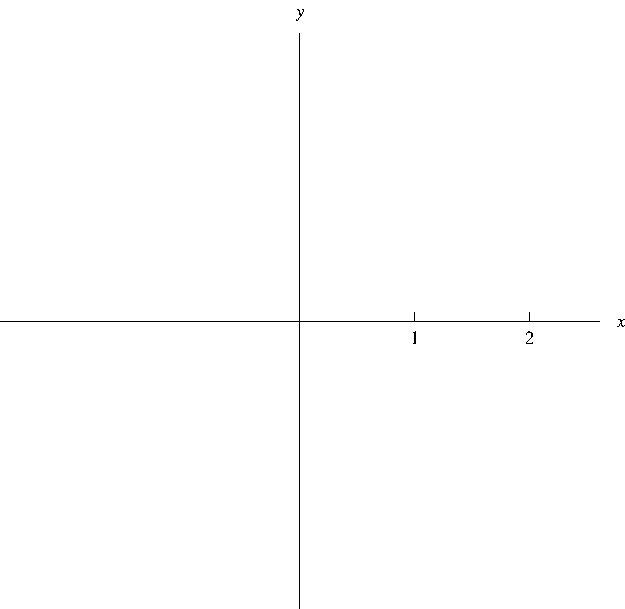
\includegraphics[height=5cm]{diff-eq-direction-fields/pictures/10-02-dirfielda.pdf}%
}%
\only<handout:0| 4>{%
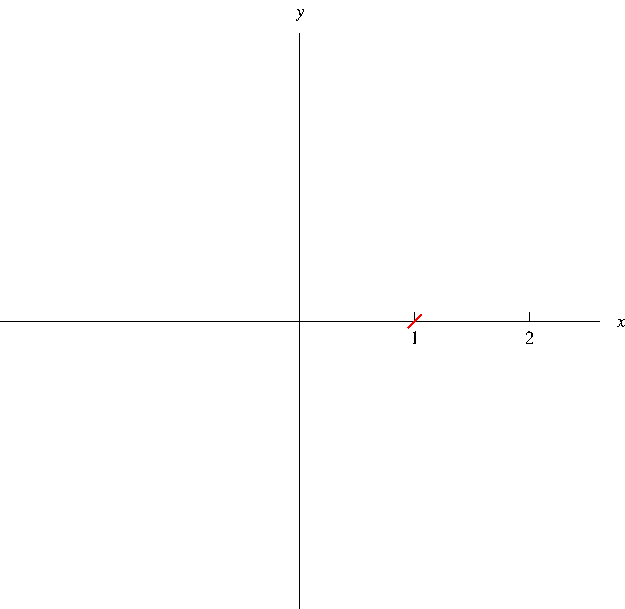
\includegraphics[height=5cm]{diff-eq-direction-fields/pictures/10-02-dirfieldb.pdf}%
}%
\only<handout:0| 5>{%
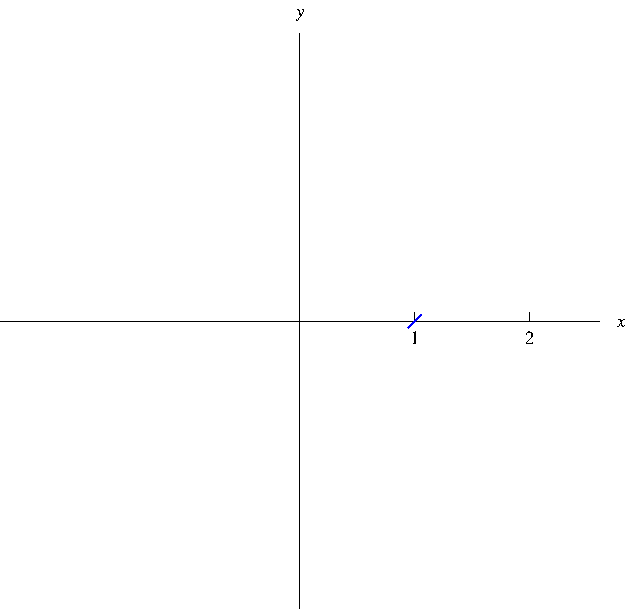
\includegraphics[height=5cm]{diff-eq-direction-fields/pictures/10-02-dirfieldc.pdf}%
}%
\only<handout:0| 6>{%
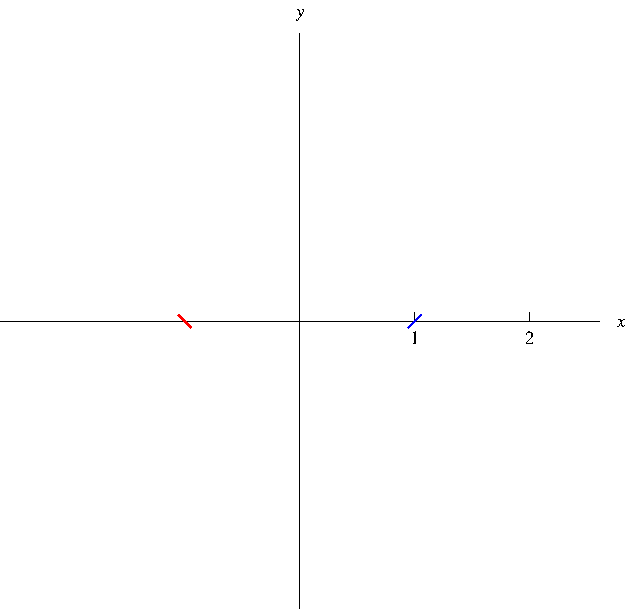
\includegraphics[height=5cm]{diff-eq-direction-fields/pictures/10-02-dirfieldd.pdf}%
}%
\only<handout:0| 7>{%
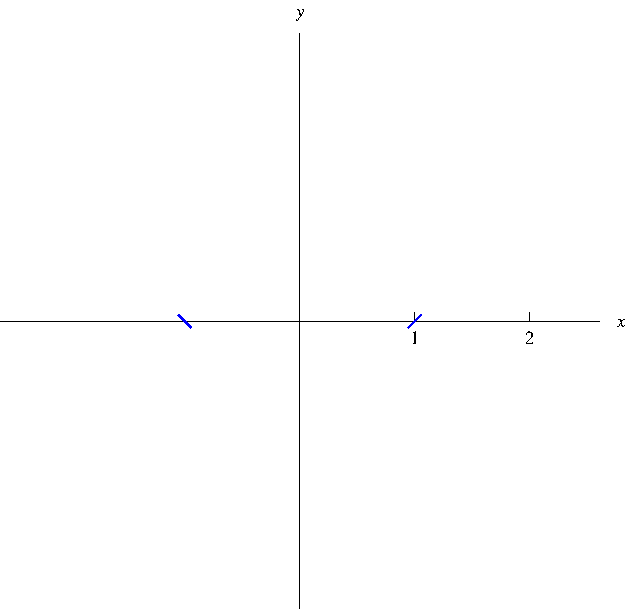
\includegraphics[height=5cm]{diff-eq-direction-fields/pictures/10-02-dirfielde.pdf}%
}%
\only<handout:0| 8>{%
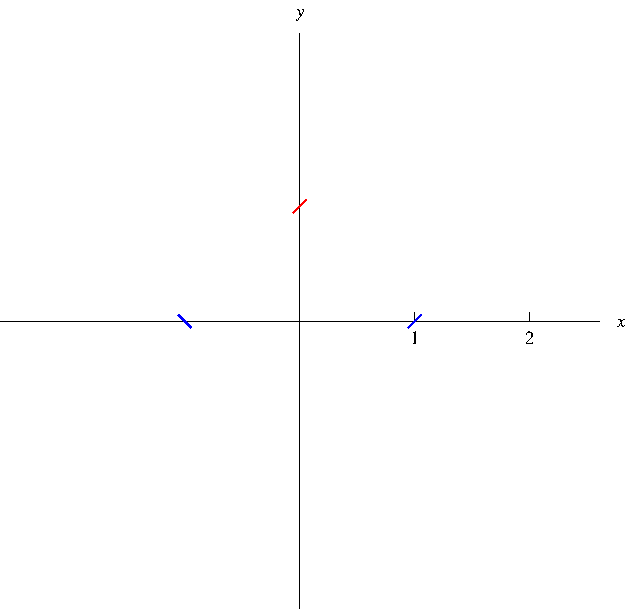
\includegraphics[height=5cm]{diff-eq-direction-fields/pictures/10-02-dirfieldf.pdf}%
}%
\only<handout:0| 9>{%
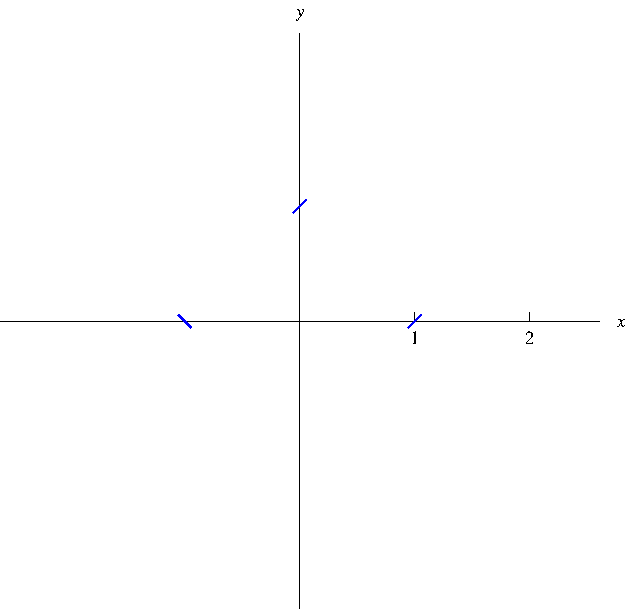
\includegraphics[height=5cm]{diff-eq-direction-fields/pictures/10-02-dirfieldg.pdf}%
}%
\only<handout:0| 10>{%
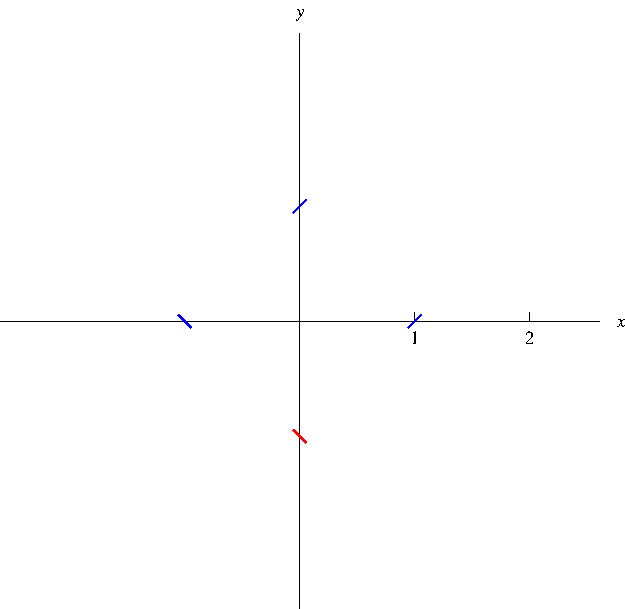
\includegraphics[height=5cm]{diff-eq-direction-fields/pictures/10-02-dirfieldh.pdf}%
}%
\only<handout:0| 11>{%
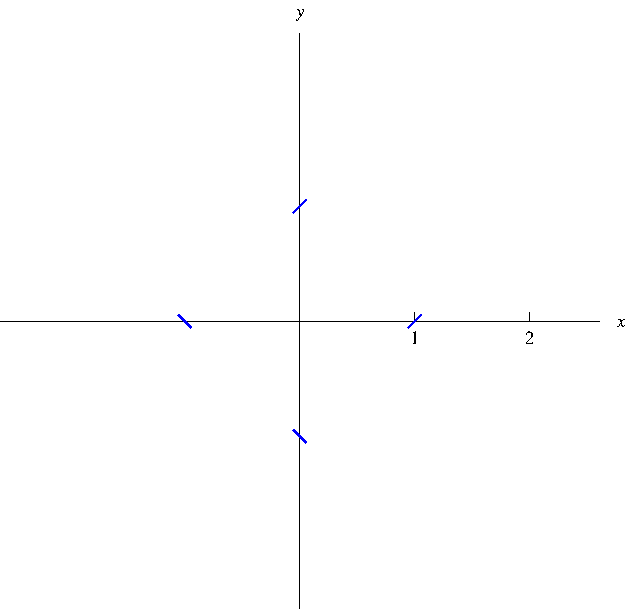
\includegraphics[height=5cm]{diff-eq-direction-fields/pictures/10-02-dirfieldi.pdf}%
}%
\only<handout:0| 12>{%
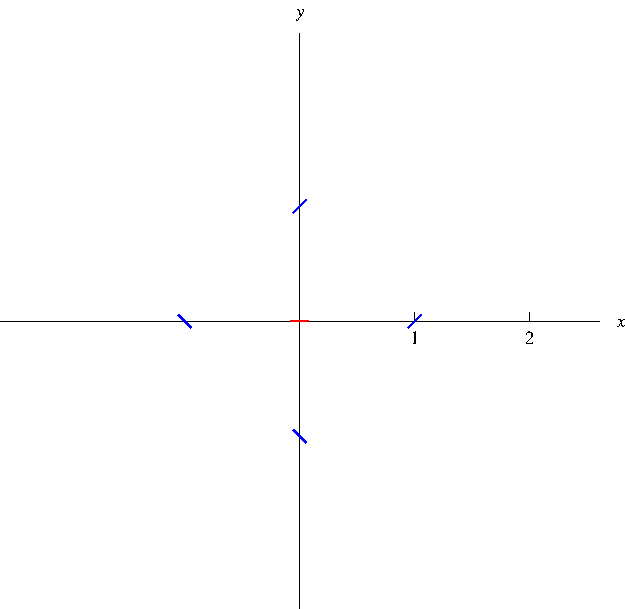
\includegraphics[height=5cm]{diff-eq-direction-fields/pictures/10-02-dirfieldj.pdf}%
}%
\only<handout:0| 13>{%
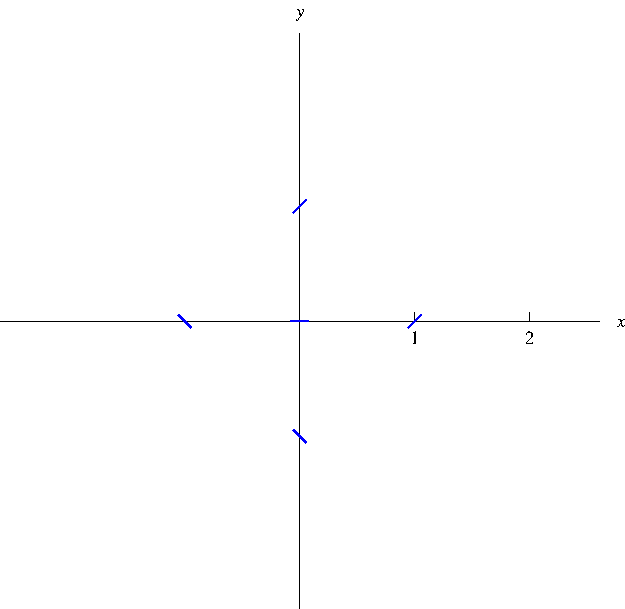
\includegraphics[height=5cm]{diff-eq-direction-fields/pictures/10-02-dirfieldk.pdf}%
}%
\only<handout:0| 14>{%
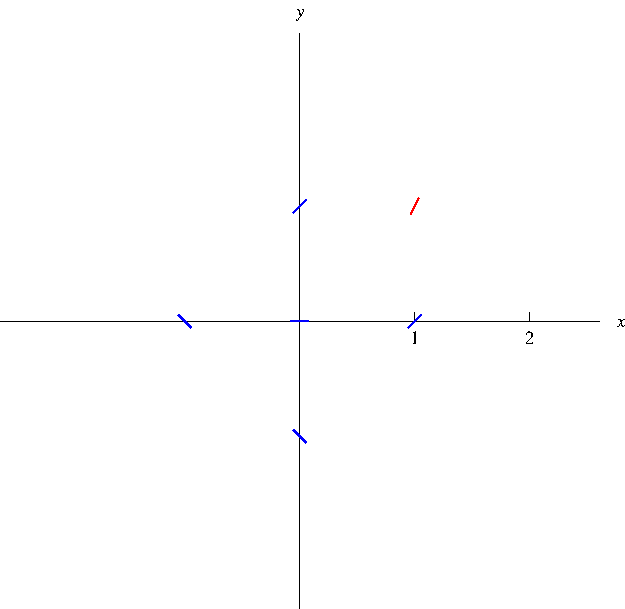
\includegraphics[height=5cm]{diff-eq-direction-fields/pictures/10-02-dirfieldl.pdf}%
}%
\only<handout:0| 15>{%
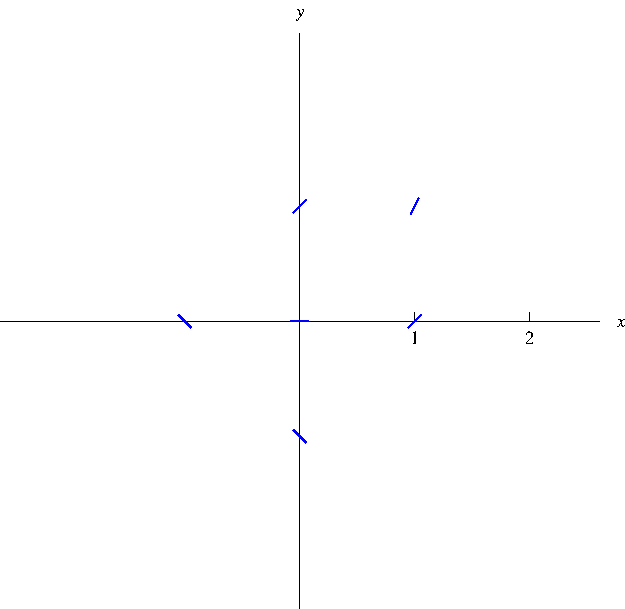
\includegraphics[height=5cm]{diff-eq-direction-fields/pictures/10-02-dirfieldm.pdf}%
}%
\only<handout:0| 16>{%
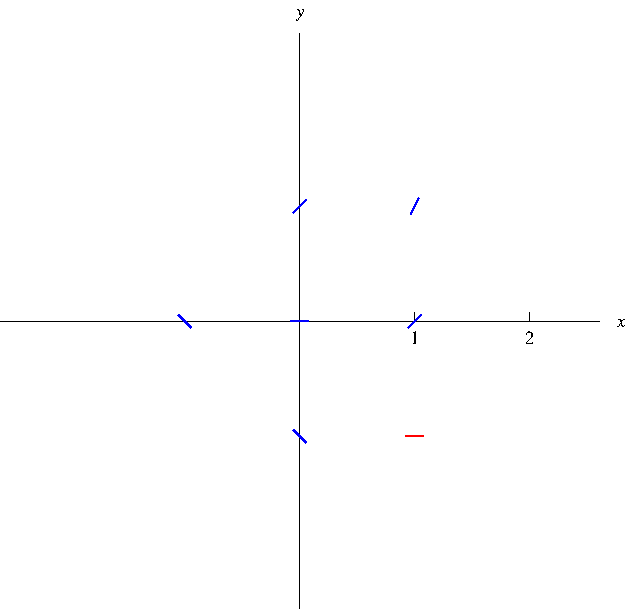
\includegraphics[height=5cm]{diff-eq-direction-fields/pictures/10-02-dirfieldn.pdf}%
}%
\only<handout:0| 17>{%
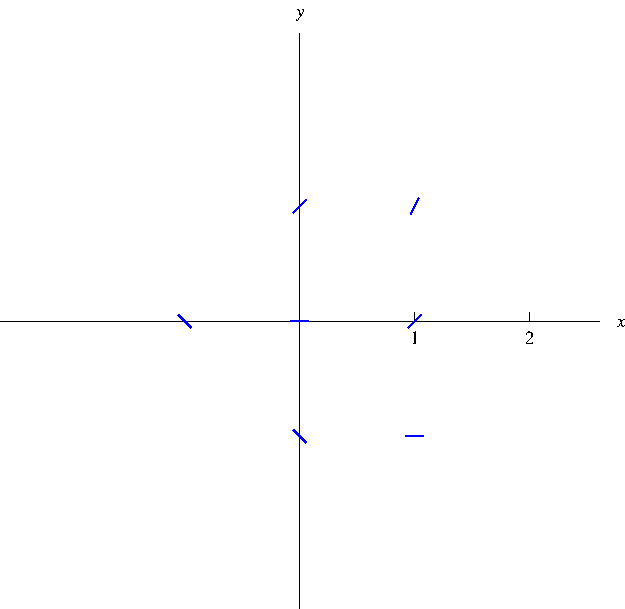
\includegraphics[height=5cm]{diff-eq-direction-fields/pictures/10-02-dirfieldo.pdf}%
}%
\only<handout:0| 18>{%
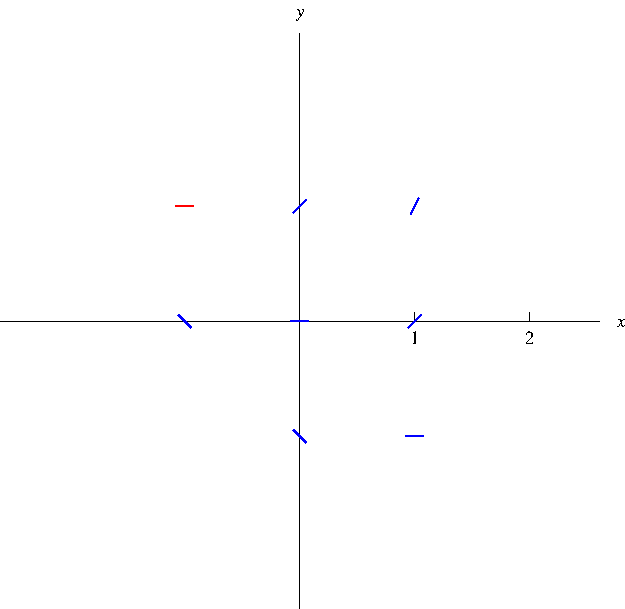
\includegraphics[height=5cm]{diff-eq-direction-fields/pictures/10-02-dirfieldp.pdf}%
}%
\only<handout:0| 19>{%
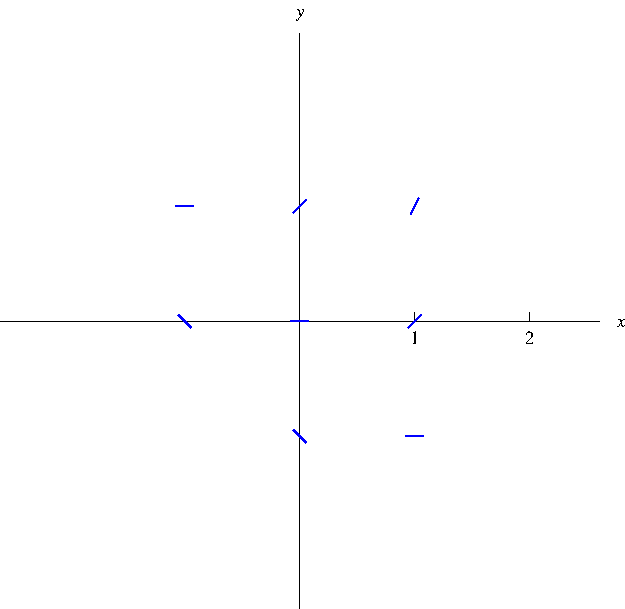
\includegraphics[height=5cm]{diff-eq-direction-fields/pictures/10-02-dirfieldq.pdf}%
}%
\only<handout:0| 20>{%
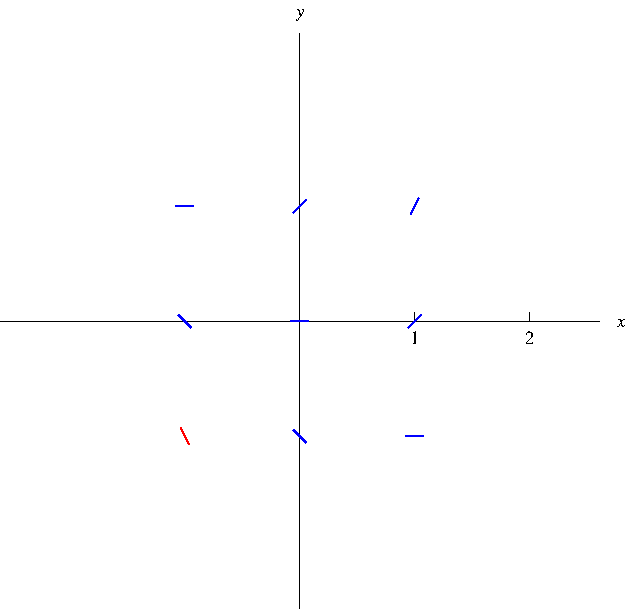
\includegraphics[height=5cm]{diff-eq-direction-fields/pictures/10-02-dirfieldr.pdf}%
}%
\only<handout:0| 21-22>{%
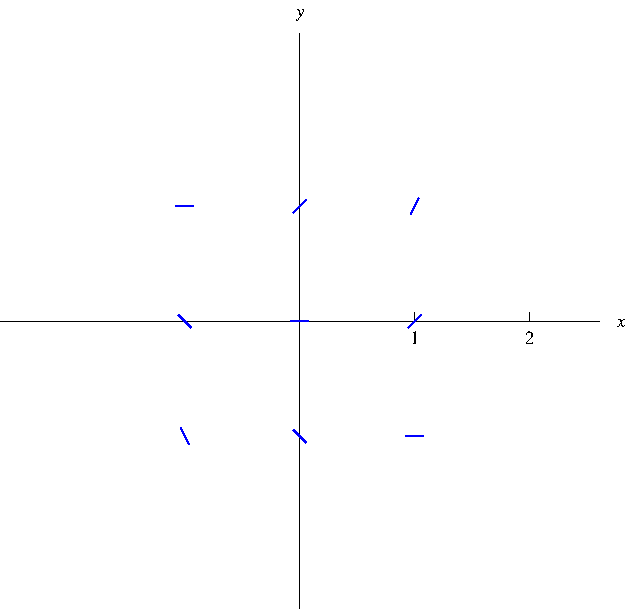
\includegraphics[height=5cm]{diff-eq-direction-fields/pictures/10-02-dirfields.pdf}%
}%
\only<handout:0| 23>{%
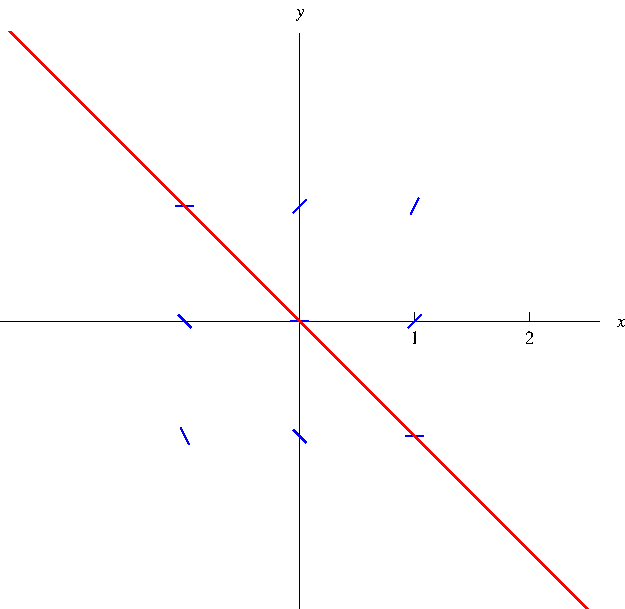
\includegraphics[height=5cm]{diff-eq-direction-fields/pictures/10-02-dirfieldt.pdf}%
}%
\only<handout:0| 24>{%
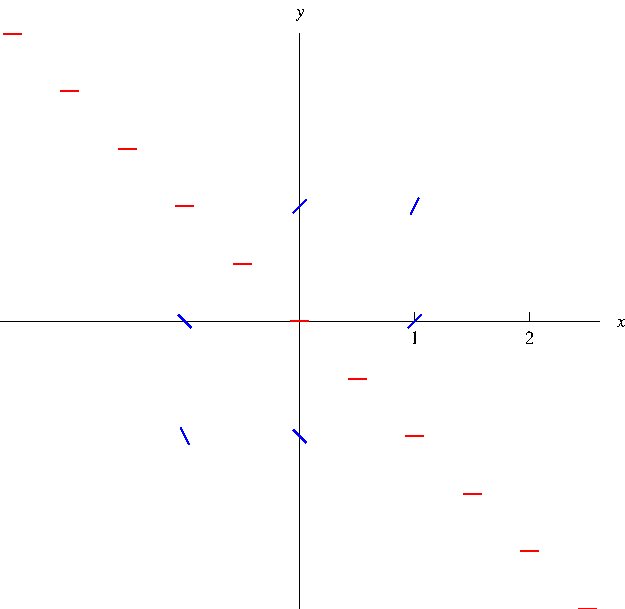
\includegraphics[height=5cm]{diff-eq-direction-fields/pictures/10-02-dirfieldu.pdf}%
}%
\only<handout:0| 25>{%
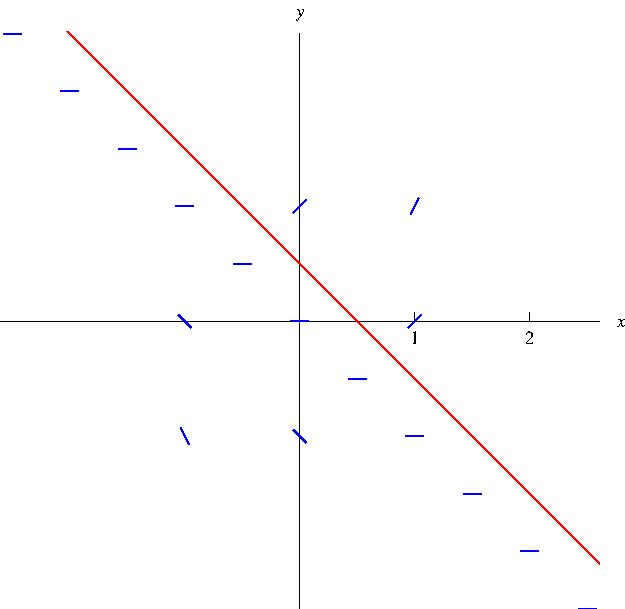
\includegraphics[height=5cm]{diff-eq-direction-fields/pictures/10-02-dirfieldv.pdf}%
}%
\only<handout:0| 26>{%
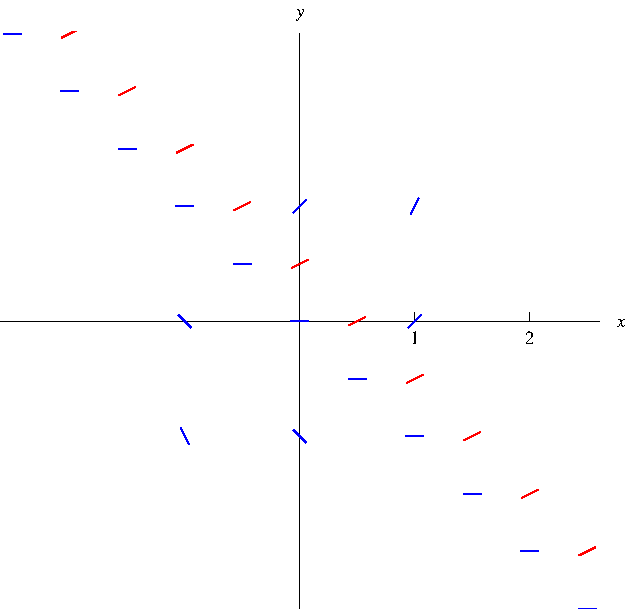
\includegraphics[height=5cm]{diff-eq-direction-fields/pictures/10-02-dirfieldw.pdf}%
}%
\only<handout:0| 27>{%
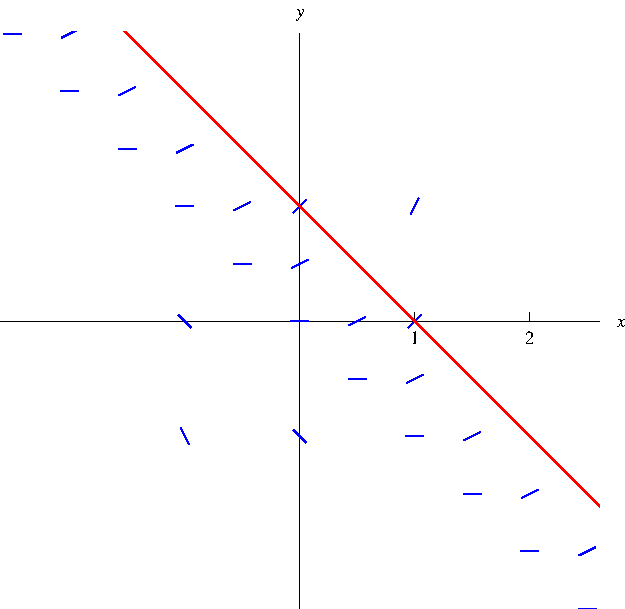
\includegraphics[height=5cm]{diff-eq-direction-fields/pictures/10-02-dirfieldx.pdf}%
}%
\only<handout:0| 28>{%
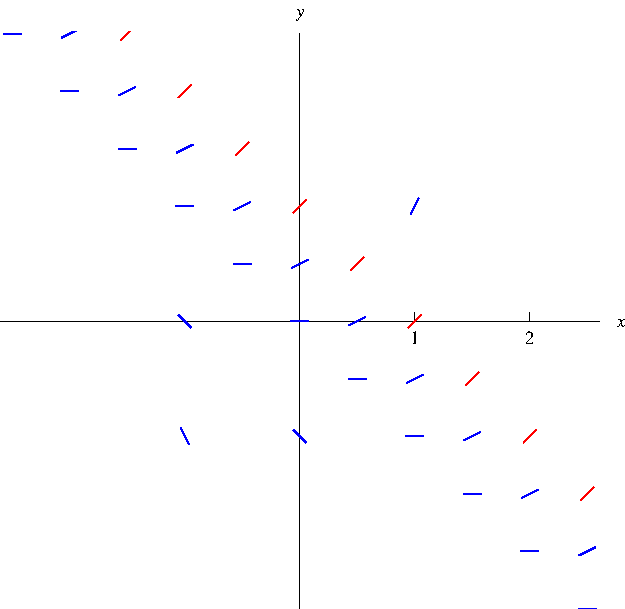
\includegraphics[height=5cm]{diff-eq-direction-fields/pictures/10-02-dirfieldy.pdf}%
}%
\only<handout:0| 29>{%
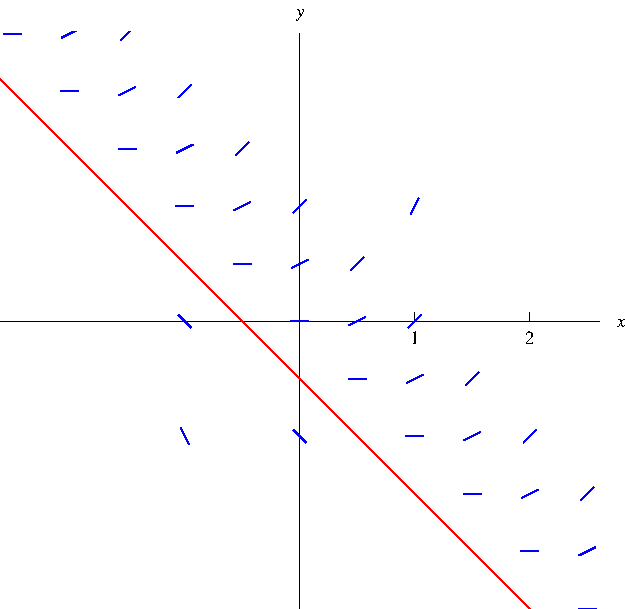
\includegraphics[height=5cm]{diff-eq-direction-fields/pictures/10-02-dirfieldz.pdf}%
}%
\only<handout:0| 30>{%
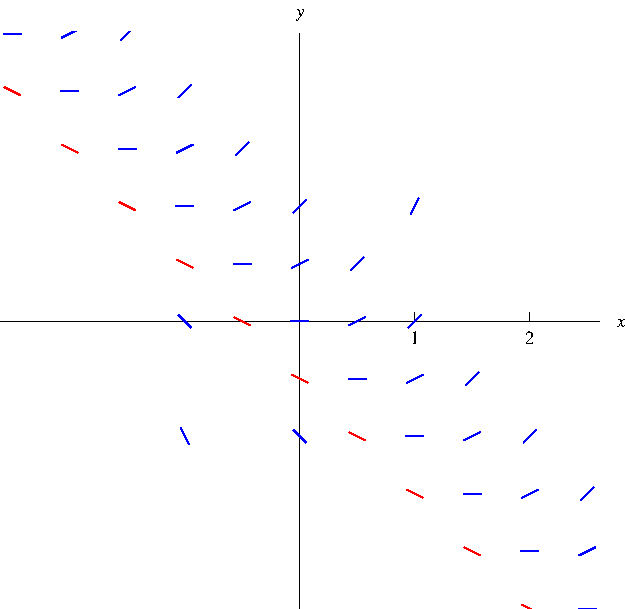
\includegraphics[height=5cm]{diff-eq-direction-fields/pictures/10-02-dirfieldaa.pdf}%
}%
\only<handout:0| 31>{%
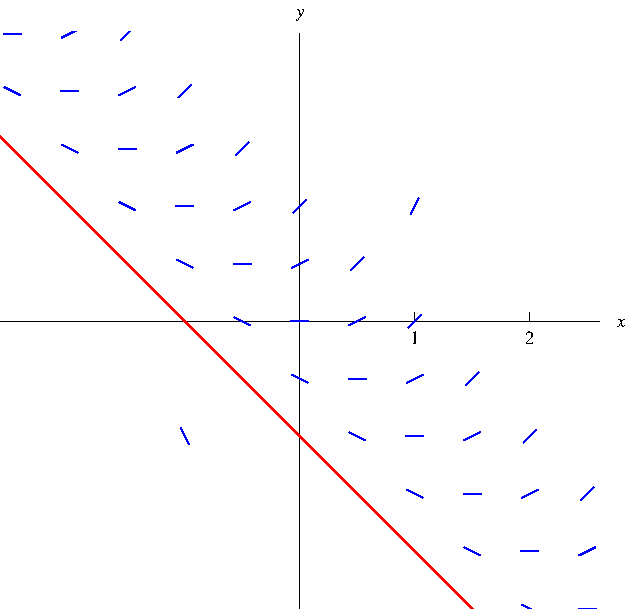
\includegraphics[height=5cm]{diff-eq-direction-fields/pictures/10-02-dirfieldab.pdf}%
}%
\only<handout:0| 32>{%
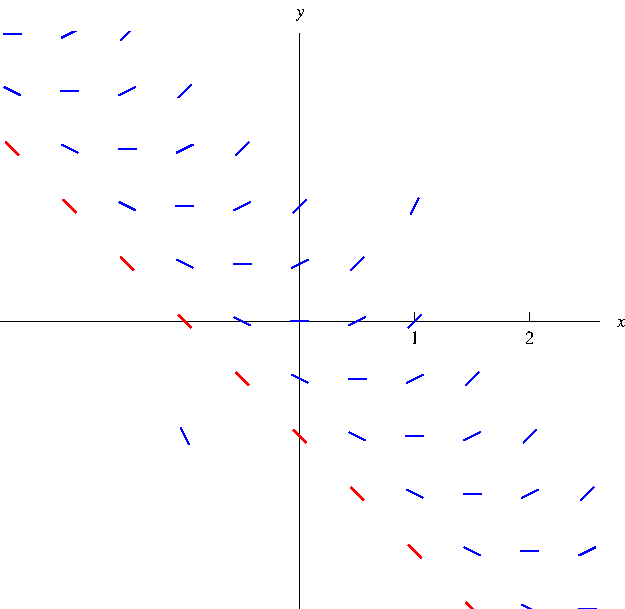
\includegraphics[height=5cm]{diff-eq-direction-fields/pictures/10-02-dirfieldac.pdf}%
}%
\only<handout:0| 33>{%
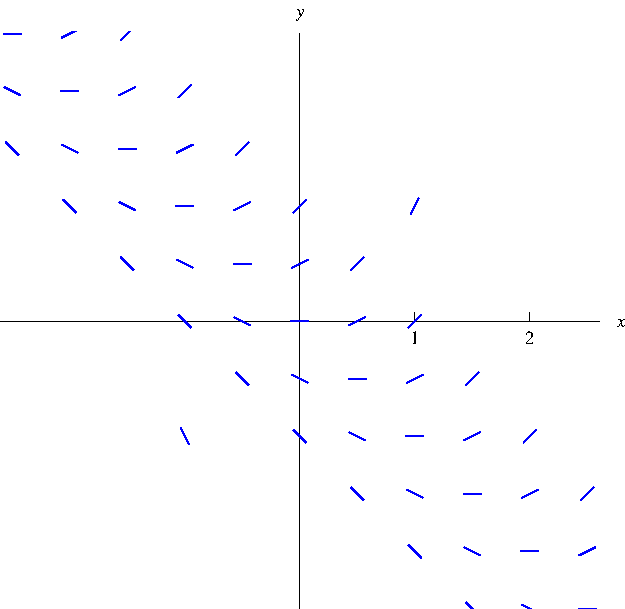
\includegraphics[height=5cm]{diff-eq-direction-fields/pictures/10-02-dirfieldad.pdf}%
}%
\only<handout:0| 34>{%
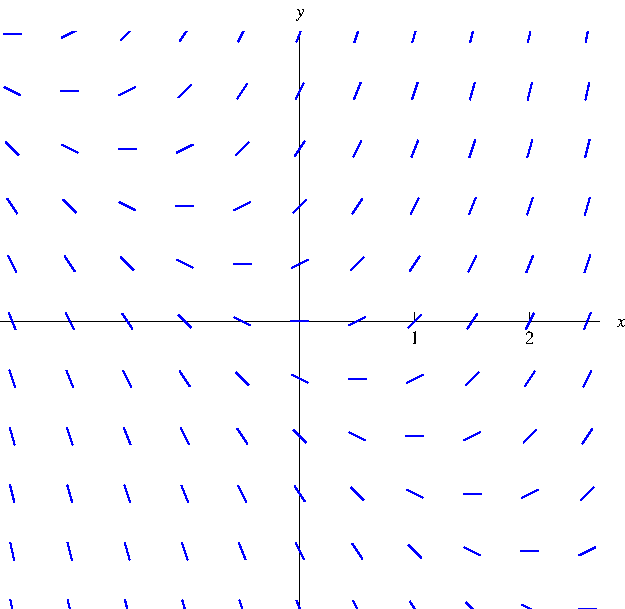
\includegraphics[height=5cm]{diff-eq-direction-fields/pictures/10-02-dirfieldae.pdf}%
}%
\only<35>{%
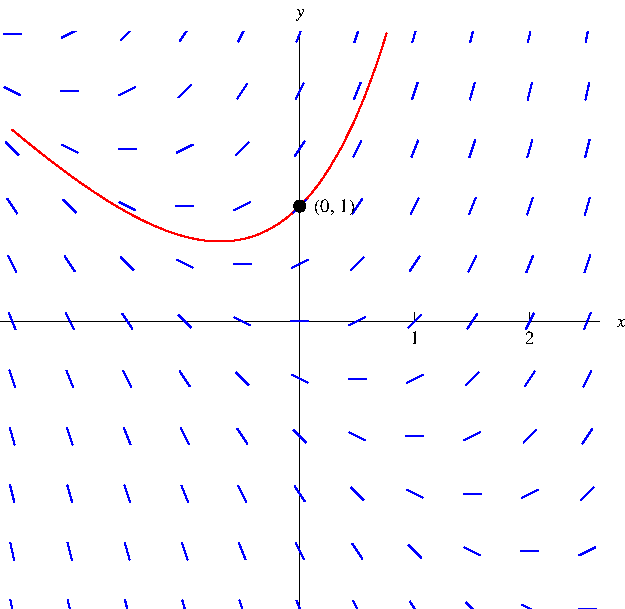
\includegraphics[height=5cm]{diff-eq-direction-fields/pictures/10-02-dirfieldaf.pdf}%
}%

\column{.3\textwidth}
\uncover<22->{%
\[%
\begin{array}{|l|r|}
\hline
\textrm{Line} & y' \\
\hline
\alert<handout:0| 23-24>{y = -x}&%
\alert<handout:0| 23-24>{\uncover<24->{0}}\\%
\alert<handout:0| 25-26>{y = -x+\frac{1}{2}}&%
\alert<handout:0| 25-26>{\uncover<26->{\frac{1}{2}}}\\%
\alert<handout:0| 27-28>{y = -x+1}&%
\alert<handout:0| 27-28>{\uncover<28->{1}}\\%
\alert<handout:0| 29-30>{y = -x-\frac{1}{2}}&%
\alert<handout:0| 29-30>{\uncover<30->{-\frac{1}{2}}}\\%
\alert<handout:0| 31-32>{y = -x-1}&%
\alert<handout:0| 31-32>{\uncover<32->{-1}}\\%
\hline
\end{array}
\]%
}%
\end{columns}
\end{frame}
% end module direction-fields-procedure

%\input{../../modules/diff-eq-direction-fields/direction-fields-ex2}
%% begin module direction-fields-ex1
\begin{frame}
\begin{example}[Example 1, p. 609]
Sketch the direction field for the differential equation $y' = x^2 + y^2 - 1$.  Use this to sketch the solution curve that passes through the origin.
\begin{columns}[c]

\column{.3\textwidth}
\uncover<2->{%
\[%
\begin{array}{|c|r|}
\hline
\textrm{Point} & y' \\
\hline
\alert<handout:0| 3-4>{(-1,1)}&%
\alert<handout:0| 3-4>{\uncover<4->{1}}\\%
\alert<handout:0| 5-6>{(0,1)}&%
\alert<handout:0| 5-6>{\uncover<6->{0}}\\%
\alert<handout:0| 7-8>{(1,1)}&%
\alert<handout:0| 7-8>{\uncover<8->{1}}\\%
\alert<handout:0| 9-10>{(-1,0)}&%
\alert<handout:0| 9-10>{\uncover<10->{0}}\\%
\alert<handout:0| 11-12>{(0,0)}&%
\alert<handout:0| 11-12>{\uncover<12->{-1}}\\%
\alert<handout:0| 13-14>{(1,0)}&%
\alert<handout:0| 13-14>{\uncover<14->{0}}\\%
\alert<handout:0| 15-16>{(-1,-1)}&%
\alert<handout:0| 15-16>{\uncover<16->{1}}\\%
\alert<handout:0| 17-18>{(0,-1)}&%
\alert<handout:0| 17-18>{\uncover<18->{0}}\\%
\alert<handout:0| 19-20>{(1,-1)}&%
\alert<handout:0| 19-20>{\uncover<20->{1}}\\%
\hline
\end{array}
\]%
}%
\column{.7\textwidth}
\ \only<handout:0| -3>{%
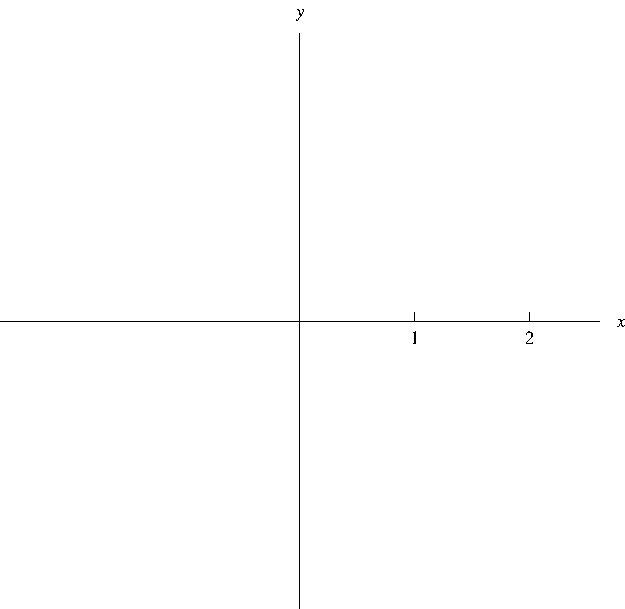
\includegraphics[height=6.5cm]{diff-eq-direction-fields/pictures/10-02-ex1a.pdf}%
}%
\only<handout:0| 4>{%
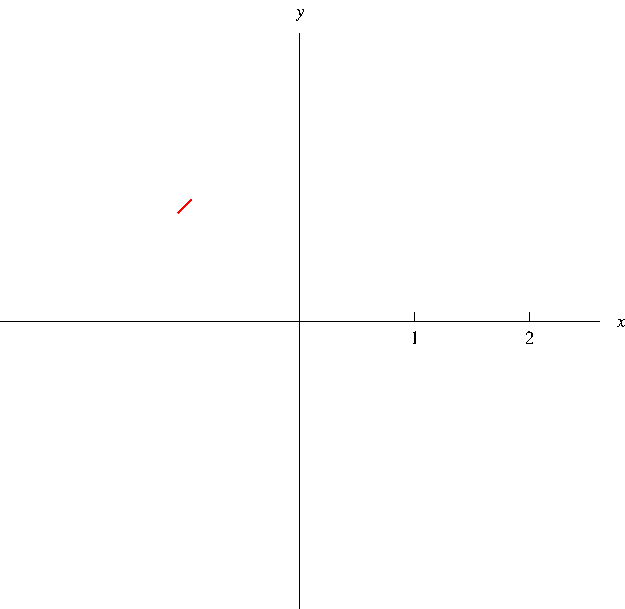
\includegraphics[height=6.5cm]{diff-eq-direction-fields/pictures/10-02-ex1b.pdf}%
}%
\only<handout:0| 5>{%
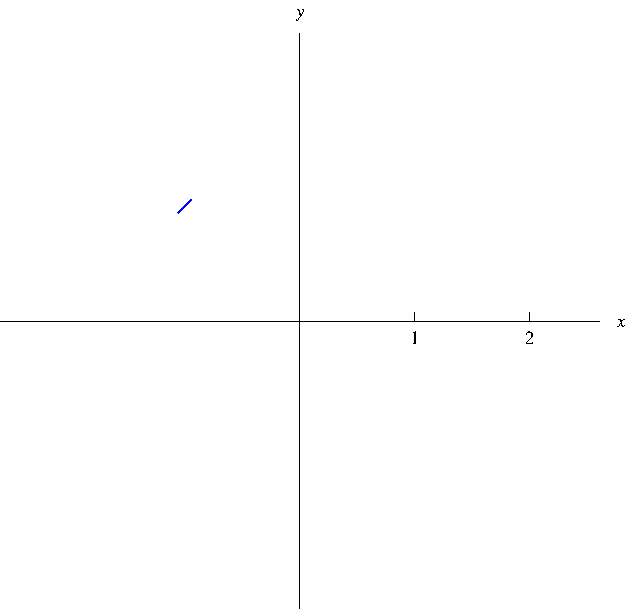
\includegraphics[height=6.5cm]{diff-eq-direction-fields/pictures/10-02-ex1c.pdf}%
}%
\only<handout:0| 6>{%
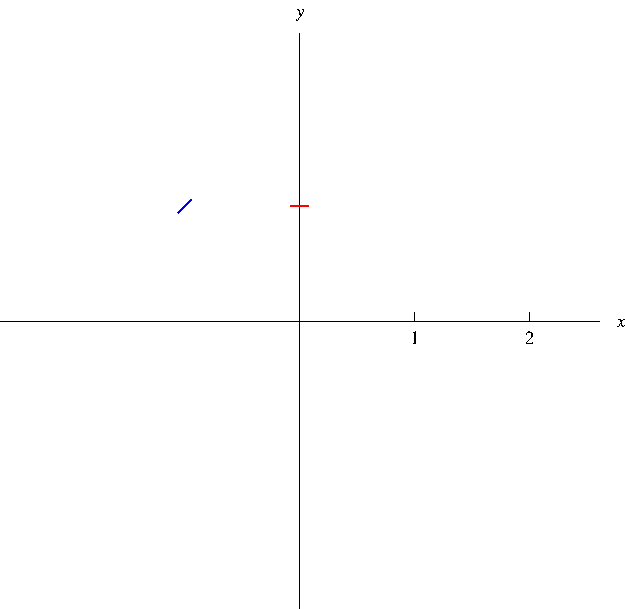
\includegraphics[height=6.5cm]{diff-eq-direction-fields/pictures/10-02-ex1d.pdf}%
}%
\only<handout:0| 7>{%
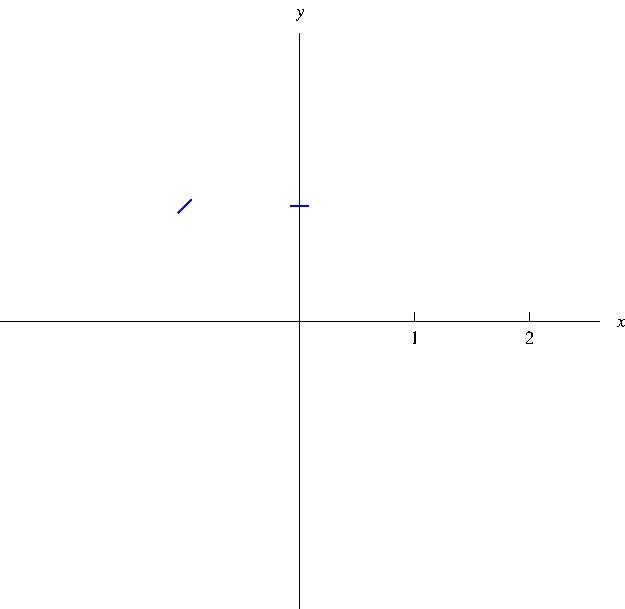
\includegraphics[height=6.5cm]{diff-eq-direction-fields/pictures/10-02-ex1e.pdf}%
}%
\only<handout:0| 8>{%
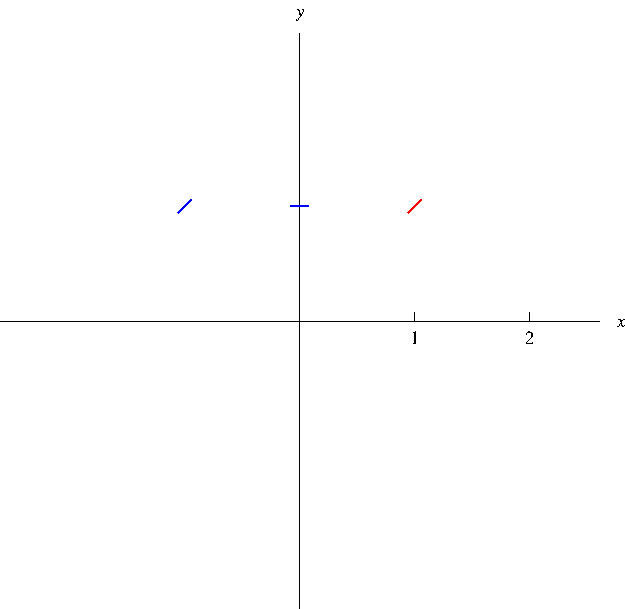
\includegraphics[height=6.5cm]{diff-eq-direction-fields/pictures/10-02-ex1f.pdf}%
}%
\only<handout:0| 9>{%
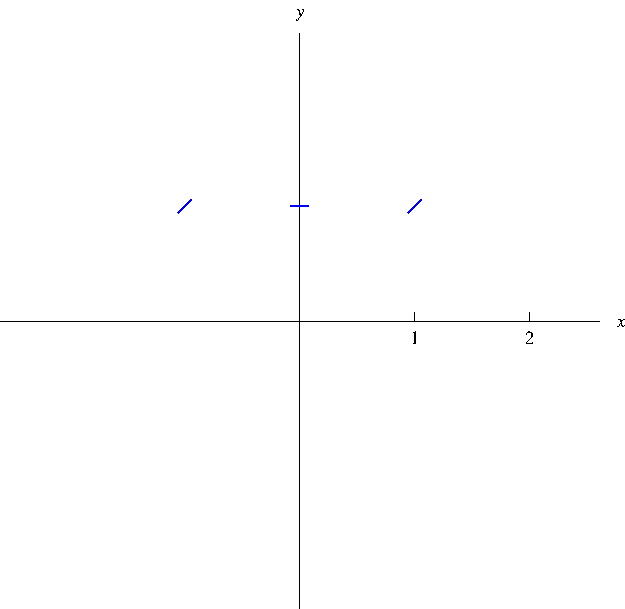
\includegraphics[height=6.5cm]{diff-eq-direction-fields/pictures/10-02-ex1g.pdf}%
}%
\only<handout:0| 10>{%
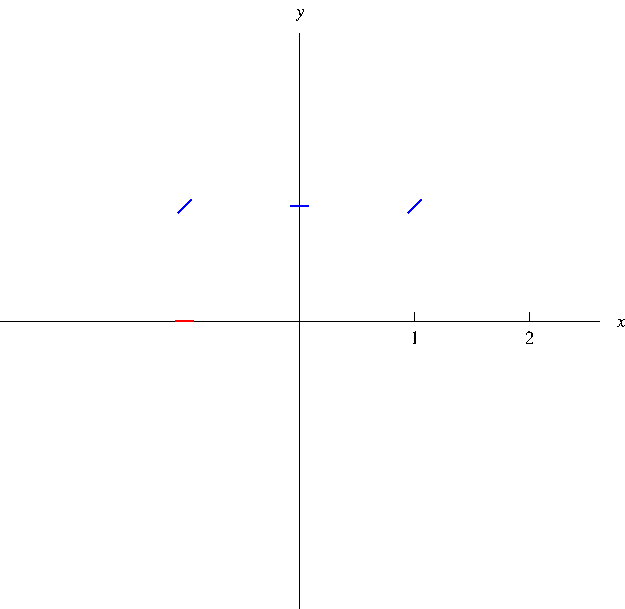
\includegraphics[height=6.5cm]{diff-eq-direction-fields/pictures/10-02-ex1h.pdf}%
}%
\only<handout:0| 11>{%
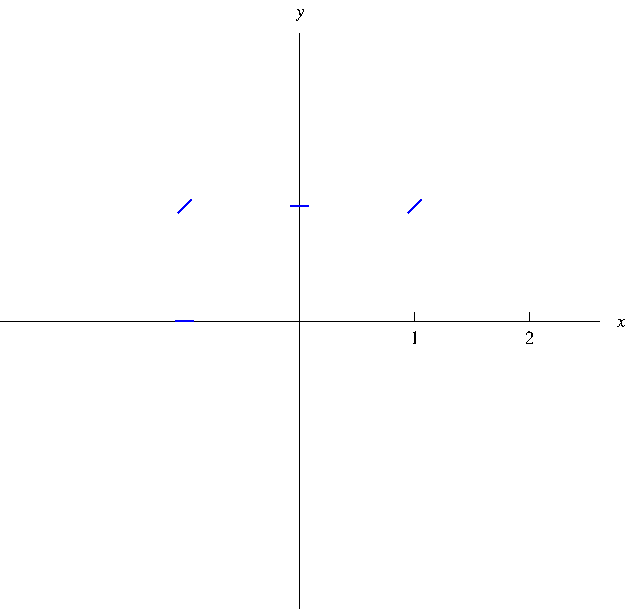
\includegraphics[height=6.5cm]{diff-eq-direction-fields/pictures/10-02-ex1i.pdf}%
}%
\only<handout:0| 12>{%
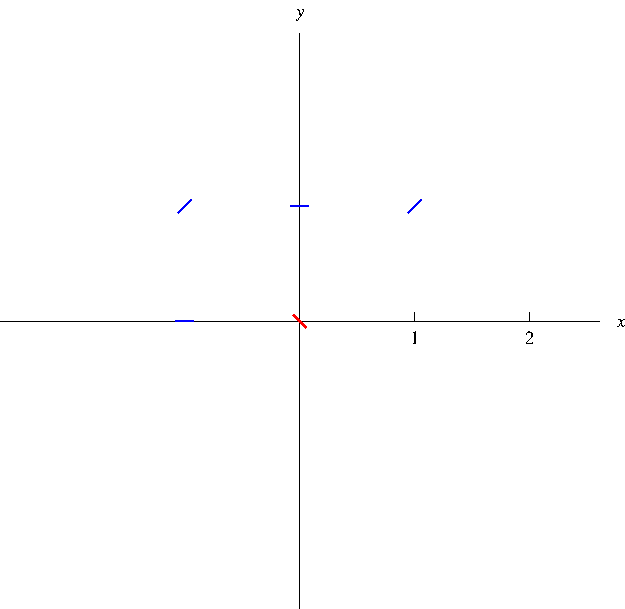
\includegraphics[height=6.5cm]{diff-eq-direction-fields/pictures/10-02-ex1j.pdf}%
}%
\only<handout:0| 13>{%
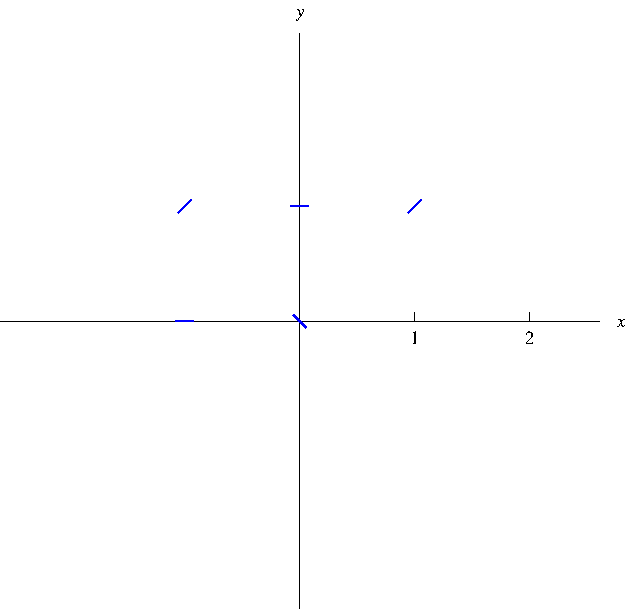
\includegraphics[height=6.5cm]{diff-eq-direction-fields/pictures/10-02-ex1k.pdf}%
}%
\only<handout:0| 14>{%
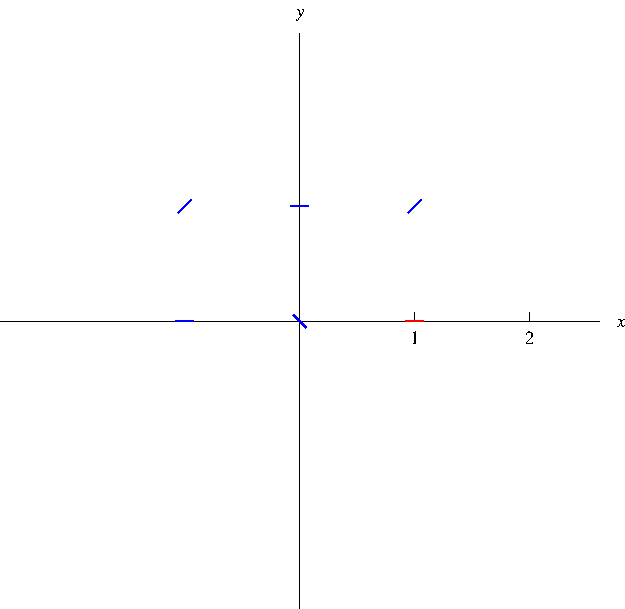
\includegraphics[height=6.5cm]{diff-eq-direction-fields/pictures/10-02-ex1l.pdf}%
}%
\only<handout:0| 15>{%
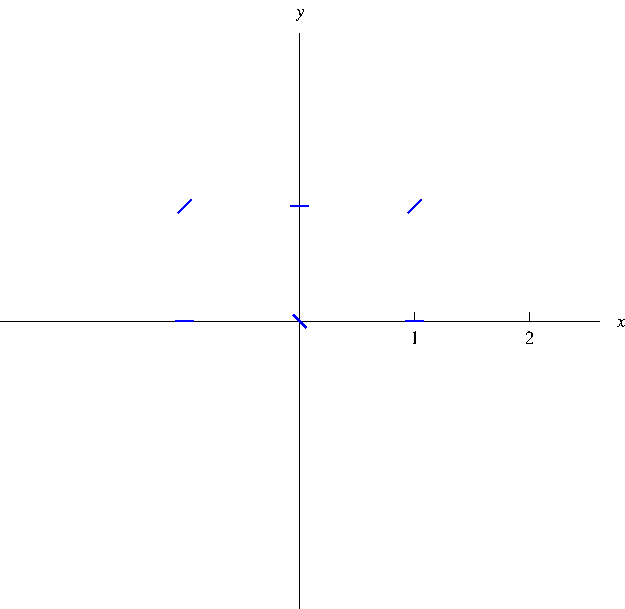
\includegraphics[height=6.5cm]{diff-eq-direction-fields/pictures/10-02-ex1m.pdf}%
}%
\only<handout:0| 16>{%
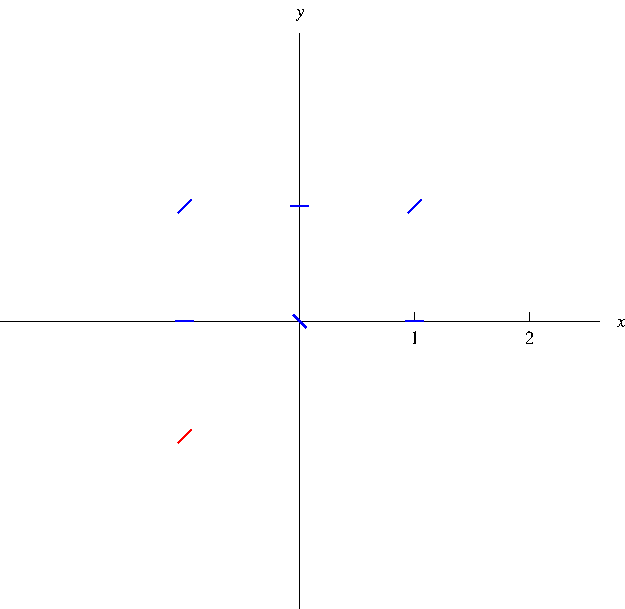
\includegraphics[height=6.5cm]{diff-eq-direction-fields/pictures/10-02-ex1n.pdf}%
}%
\only<handout:0| 17>{%
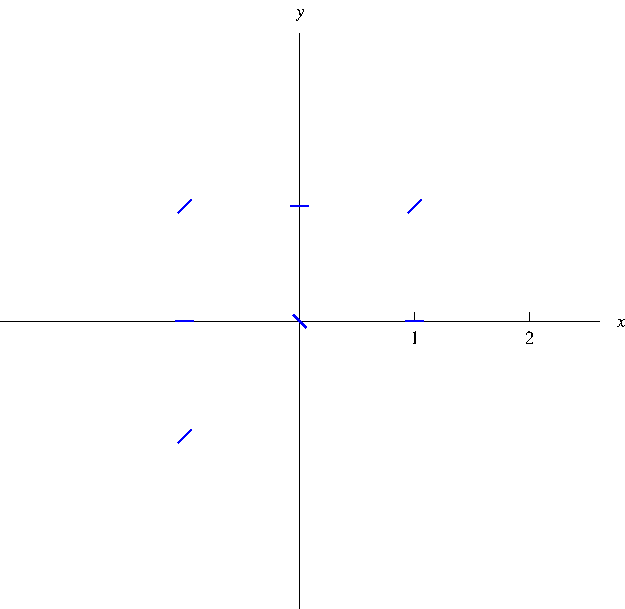
\includegraphics[height=6.5cm]{diff-eq-direction-fields/pictures/10-02-ex1o.pdf}%
}%
\only<handout:0| 18>{%
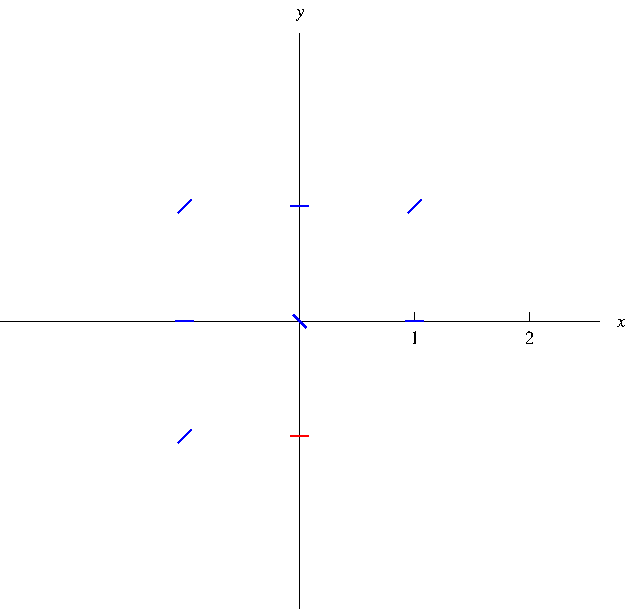
\includegraphics[height=6.5cm]{diff-eq-direction-fields/pictures/10-02-ex1p.pdf}%
}%
\only<handout:0| 19>{%
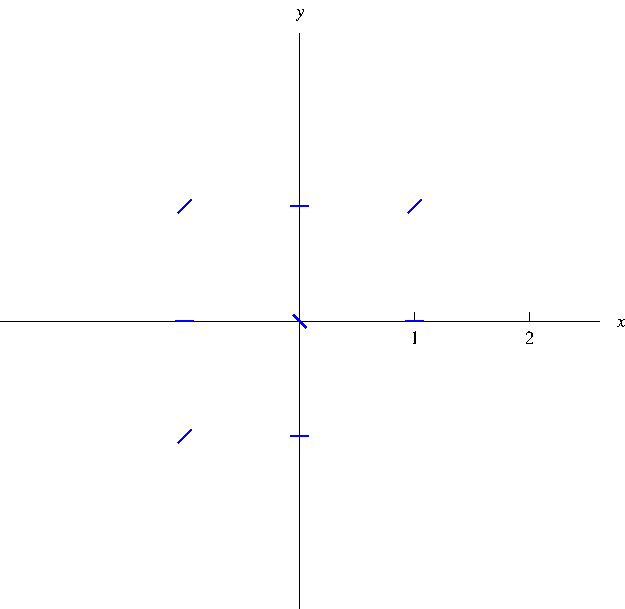
\includegraphics[height=6.5cm]{diff-eq-direction-fields/pictures/10-02-ex1q.pdf}%
}%
\only<handout:0| 20>{%
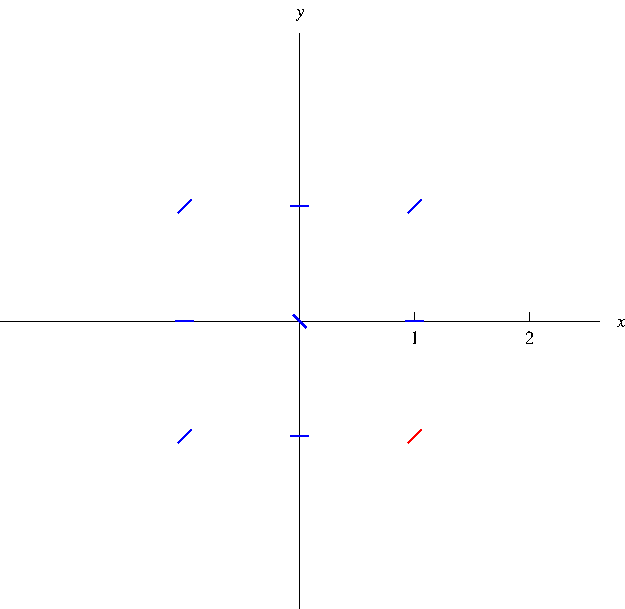
\includegraphics[height=6.5cm]{diff-eq-direction-fields/pictures/10-02-ex1r.pdf}%
}%
\only<handout:0| 21>{%
\includegraphics[height=6.5cm]{diff-eq-direction-fields/pictures/10-02-ex1s.pdf}%
}%
\only<handout:0| 22>{%
\includegraphics[height=6.5cm]{diff-eq-direction-fields/pictures/10-02-ex1t.pdf}%
}%
\only<23->{%
\includegraphics[height=6.5cm]{diff-eq-direction-fields/pictures/10-02-ex1u.pdf}%
}%
\end{columns}
\end{example}
\end{frame}
% end module direction-fields-ex1

%% begin module diff-eq-separable-def
\begin{frame}
\frametitle{(10.3) Separable Equations}
In this section, we will discuss a type of differential equation, called a separable equation, for which it is possible to find an explicit solution.

\begin{definition}[Separable Equation]
A separable equation is a first-order equation in which the expression for $\diff y/\diff x$ can be factored as a function of $x$ times a function of $y$.  In other words,
\[
\frac{\diff y}{\diff x} = g(x)f(y).
\]
\end{definition}

\uncover<2->{%
Let $f(y) = 1/h(y)$.  Then
\[
\frac{\diff y}{\diff x} = \frac{g(x)}{h(y)}.
\]
}%
\end{frame}
% end module diff-eq-separable-def

%% begin module diff-eq-separable-solution
\begin{frame}
\[
\frac{\diff y}{\diff x} = \frac{g(x)}{h(y)}.
\]
\begin{itemize}
\item<2->  To solve, write this in differential form:
\uncover<2->{%
\abovedisplayskip=0pt
\belowdisplayshortskip=0pt
\belowdisplayskip=0pt
\[
h(y) \diff y = g(x)\diff x
\]
}%
\item<3->  Now integrate:
\uncover<3->{%
\abovedisplayskip=0pt
\belowdisplayshortskip=0pt
\belowdisplayskip=0pt
\[
\int h(y) \diff y = \int g(x)\diff x
\]
}%
\item<4->  This defines $y$ implicitly as a function of $x$.
\item<5->  Sometimes we might be able to solve explicitly for $y$ in terms of $x$.
\end{itemize}
\end{frame}

\begin{frame}
Why does this process yield a function that satisfies the original differential equation?  Suppose that $\int h(y) \diff y = \int g(x) \diff x$.  Then we will use the Chain Rule to show that $y$ satisfies the original equation.
\begin{eqnarray*}
\int h(y) \diff y & = & \int g(x) \diff x\\
\uncover<2->{%
\frac{\diff}{\diff x}\left( \int h(y)\diff y\right)%
}%
& \uncover<2->{ = } &%
\uncover<2->{%
\frac{\diff}{\diff x}\left( \int g(x)\diff x\right)%
}\\%
\uncover<3->{%
\frac{\diff}{\diff y}\left( \int h(y)\diff y\right)\frac{\diff  y}{\diff x}%
}%
& \uncover<3->{ = } &%
\uncover<3->{%
\frac{\diff}{\diff x}\left( \int g(x)\diff x\right)%
}\\%
\uncover<4->{%
h(y) \frac{\diff y}{\diff x}%
}%
& \uncover<4->{ = } &%
\uncover<4->{%
g(x)%
}\\%
\frac{\diff y}{\diff x} & = & \frac{g(x)}{h(y)}
\end{eqnarray*}
\end{frame}
% end module diff-eq-separable-solution

%% begin module diff-eq-separable-ex1
\begin{frame}
\begin{example}[Example 1, p. 617]
Solve the differential equation $\frac{\diff y}{\diff x} = \frac{x^2}{y^2}$, and find the solution that satisfies the intial condition $y(0) = 2$.
\belowdisplayskip=0pt
\begin{eqnarray*}
\uncover<2->{%
y^2 \diff y %
}%
& \uncover<2->{ = } &%
\uncover<2->{%
x^2 \diff x %
}\\%
\uncover<3->{%
\int y^2 \diff y %
}%
& \uncover<3->{ = } &%
\uncover<3->{%
\int x^2 \diff x %
}\\%
\uncover<4->{%
\frac{y^3}{3}%
}%
& \uncover<4->{ = } &%
\uncover<4->{%
\frac{x^3}{3} + C
}\\%
\uncover<5->{%
y%
}%
& \uncover<5->{ = } &%
\uncover<5->{%
\sqrt[3]{x^3 + 3C}%
}\\%
\uncover<6->{%
y%
}%
& \uncover<6->{ = } &%
\uncover<6->{%
\sqrt[3]{x^3 + K}%
}%
\end{eqnarray*}
\uncover<7->{%
To find the solution satisfying the initial condition, set $2 = y(0) = \sqrt[3]{0^3 + K} = \sqrt[3]{K}$.  %
}%
\uncover<8->{%
Then $\sqrt[3]{K} = 2$, so $K = 8$.%
}%
\uncover<9->{%
\belowdisplayskip=0pt
\abovedisplayskip=0pt
\[
y = \sqrt[3]{x^3 + 8}.
\]
}%
\end{example}
\end{frame}
% end module diff-eq-separable-ex1

%% begin module diff-eq-separable-ex3
\begin{frame}
\begin{example}[Example 3, p. 617]
Solve the equation $\alert<handout:0| 9>{y' =} \alert<handout:0| 9>{x^2y}$.
\belowdisplayskip=0pt
\abovedisplayskip=0pt
\begin{eqnarray*}
\uncover<2->{%
\frac{\diff y}{\diff x}%
}%
& \uncover<2->{ = } &%
\uncover<2->{%
x^2y%
}\\%
\uncover<3->{%
\frac{1}{y}\diff y%
}%
& \uncover<3->{ = } &%
\uncover<3->{%
x^2\diff x \qquad y\neq 0%
}\\%
\uncover<4->{%
\int \frac{1}{y}\diff y%
}%
& \uncover<4->{ = } &%
\uncover<4->{%
\int x^2\diff x%
}\\%
\uncover<5->{%
\ln |y|%
}%
& \uncover<5->{ = } &%
\uncover<5->{%
\frac{1}{3}x^3 + C%
}\\%
\uncover<6->{%
e^{\ln |y|}%
}%
& \uncover<6->{ = } &%
\uncover<6->{%
e^{x^3/3 + C}%
}\\%
\uncover<7->{%
\alert<handout:0| 8>{|}y\alert<handout:0| 8>{|}%
}%
& \uncover<7->{ = } &%
\uncover<7->{%
e^Ce^{x^3/3}%
}\\%
\uncover<8->{%
y%
}%
& \uncover<8->{ = } &%
\uncover<8->{%
\alert<handout:0| 8,10>{\pm} \alert<handout:0| 10>{e^C}e^{x^3/3}%
}%
\end{eqnarray*}
\uncover<9->{%
The function $y = 0$ satisfies the equation.  }%
\uncover<10->{ General solution:
\belowdisplayskip=0pt
\abovedisplayskip=0pt
\[
y = \alert<handout:0| 10>{A}e^{x^3/3}.
\]
\vspace{-.2in}
}%
\end{example}
\end{frame}
% end module diff-eq-separable-ex3

%% begin module orthogonal-trajectory-def
\begin{frame}
\frametitle{Orthogonal Trajectories}
\begin{definition}[Orthogonal Trajectory]
An orthogonal trajectory to a family of curves is a curve that intersects each curve of the family orthogonally (that is, at right angles).
\end{definition}

\begin{columns}[c]
\column{.5\textwidth}
\ \uncover<2->{%
\includegraphics[height=5.5cm]{diff-eq-separable/pictures/10-03-orthcirc.pdf}%
}%
\column{.5\textwidth}
\uncover<2->{%
Each member of the family $y = mx$ of straight lines passing through the origin is an orthogonal trajectory to the family $x^2 + y^2 = r^2$ of circles centered at the origin.
}%
\end{columns}
\end{frame}
% end module orthogonal-trajectory-def

%% begin module orthogonal-trajectory-ex5
\begin{frame}
\begin{example}
Find the orthogonal trajectories of the family $x = ky^2$, where $k$ is an arbitrary constant.  \uncover<3->{\alert<handout:0| 3>{Differentiate implicitly:}}
\begin{columns}[c]
\column{.5\textwidth}
\abovedisplayskip=0pt
\belowdisplayskip=0pt
\begin{eqnarray*}
\uncover<2->{%
\alert<handout:0| 5>{x}%
}%
& \uncover<2->{ \alert<handout:0| 5>{=} } &%
\uncover<2->{%
\alert<handout:0| 5>{ky^2}%
}\\%
\uncover<3->{%
1%
}%
& \uncover<3->{ = } &%
\uncover<3->{%
2\alert<handout:0| 4-5>{k}y\frac{\diff y}{\diff x}%
}\\%
\uncover<4->{%
1%
}%
& \uncover<4->{ = } &%
\uncover<4->{%
2\left(\alert<handout:0| 4-5>{\uncover<5->{\frac{x}{y^2}}}\right) y\frac{\diff y}{\diff x}%
}\\%
\uncover<6->{%
\frac{\diff y}{\diff x}%
}%
& \uncover<6->{ = } &%
\uncover<6->{%
\frac{y}{2x}%
}%
\end{eqnarray*}
%\begin{center}

\hfil\hfil\psset{xunit=0.4cm, yunit=0.4cm}
\begin{pspicture}(-4.4, -3.228427)(4.4,3.317125)
\tiny
\fcAxesStandard{-4.15}{-2.978427}{4.15}{2.967125}
%Calculator input: plotCurve{}(1/2 t^{2}, t, - (8)^{1/2}, (8)^{1/2})
\parametricplot[linecolor=\fcColorGraph, plotpoints=1000]{-2.82843}{2.82843}{t 2 exp 0.5 mul t}
%Calculator input: plotCurve{}(-1/2 t^{2}, t, - (8)^{1/2}, (8)^{1/2})
\parametricplot[linecolor=\fcColorGraph, plotpoints=1000]{-2.82843}{2.82843}{t 2 exp -0.5 mul t}
%Calculator input: plotCurve{}(t^{2}, t, - (4)^{1/2}, (4)^{1/2})
\parametricplot[linecolor=\fcColorGraph, plotpoints=1000]{-2}{2}{t 2 exp t}
%Calculator input: plotCurve{}(- t^{2}, t, - (4)^{1/2}, (4)^{1/2})
\parametricplot[linecolor=\fcColorGraph, plotpoints=1000]{-2}{2}{t 2 exp -1 mul t}
%Calculator input: plotCurve{}(-2 t^{2}, t, - (2)^{1/2}, (2)^{1/2})
\parametricplot[linecolor=\fcColorGraph, plotpoints=1000]{-1.41421}{1.41421}{t 2 exp -2 mul t}
%Calculator input: plotCurve{}(2 t^{2}, t, - (2)^{1/2}, (2)^{1/2})
\parametricplot[linecolor=\fcColorGraph, plotpoints=1000]{-1.41421}{1.41421}{t 2 exp 2 mul t}
\uncover<11->{%
%Calculator input: plotCurve{}(1/2 \cos{}t, 1/2\sqrt{2} \sin{}t, 0, 2 \pi)
\parametricplot[linecolor=blue, plotpoints=1000]{0}{6.28319}{t 57.29578 mul cos 0.5 mul t 57.29578 mul sin 0.707107 mul }%
%Calculator input: plotCurve{}(3/2 \cos{}t, 3/2\sqrt{2} \sin{}t, 0, 2 \pi)
\parametricplot[linecolor=blue, plotpoints=1000]{0}{6.28319}{t 57.29578 mul cos 1.5 mul t 57.29578 mul sin 2.12132 mul }%
%Calculator input: plotCurve{}(\cos{}t, \sqrt{2} \sin{}t, 0, 2 \pi)
\parametricplot[linecolor=blue, plotpoints=1000]{0}{6.28319}{t 57.29578 mul cos t 57.29578 mul sin 1.414214 mul }%
}%
%\fcFullDot{1.081139}{1.470469}
\end{pspicture}

%\end{center}
\column{.5\textwidth}
\uncover<7->{%
An orthogonal trajectory will have a slope that is the negative reciprocal of the slope of the curve.
}%
\abovedisplayskip=0pt
\belowdisplayskip=0pt
\begin{eqnarray*}
\uncover<7->{%
\frac{\diff y}{\diff x}%
}%
& \uncover<7->{ = } &%
\uncover<7->{%
-\frac{2x}{y}%
}\\%
\uncover<8->{%
\int y \diff y%
}%
& \uncover<8->{ = } &%
\uncover<8->{%
-\int 2x\diff x%
}\\%
\uncover<9->{%
\frac{y^2}2%
}%
& \uncover<9->{ = } &%
\uncover<9->{%
-x^2 + C%
}\\%
\uncover<10->{%
x^2 + \frac{y^2}{2} %
}%
& \uncover<10->{ = } &%
\uncover<10->{%
C%
}%
\end{eqnarray*}
\uncover<11->{%
The ellipses $x^2 + \frac{y^2}{2} = C$ are all orthogonal trajectories to $x = ky^2$.
}%
\end{columns}
\end{example}
\end{frame}
% end module orthogonal-trajectory-ex5

%% begin module mixing-problem-intro
\begin{frame}
\frametitle{Mixing Problems}
\begin{itemize}
\item  Typical mixing problems involve:
\item  A tank of fixed capacity.
\item  A completely mixed solution of some substance in the tank.
\item  A solution of a certain concentration enters the tank at a fixed rate.
\item  In the tank, the solution immediately becomes completely stirred.
\item  The mixture leaves at the other end at a fixed rate (possibly a different rate).
\item<2->  Let $y(t)$ denote the amount of substance in the tank at time $t$.
\item<2->  Then $y'(t)$ denotes the rate at which the substance is being added minus the rate at which it is being removed.
\item<2->  This often gives a differential equation.
\end{itemize}
\end{frame}
% end module mixing-problem-intro

%% begin module mixing-problem-ex6
\begin{frame}[t]
\begin{example}[Example 6, p. 621]
\alert<handout:0| 5>{A tank contains 20 kg of salt} dissolved in 5000 L of water.  \alert<handout:0| 11>{Brine that contains 0.03 kg of salt per liter of water enters the tank} \alert<handout:0| 13>{at a rate of 25 L/min}.  \alert<handout:0| 16>{The solution is kept thoroughly mixed} and \alert<handout:0| 18>{drains from the tank at the same rate}.  \alert<handout:0| 7>{How much salt is in the tank after half an hour?}
\begin{itemize}
\item<2->  Let $y(t)$ denote the amount of salt (in kg) after $t$ minutes.
\item<3->  \alert<handout:0| 4-5>{Given: $y(0) = \uncover<5->{20.}$}  \alert<handout:0| 6-7>{We want to know: $\uncover<7->{y(30).}$}
\end{itemize}
\abovedisplayskip=0pt
\belowdisplayskip=0pt
\begin{eqnarray*}
\uncover<8->{%
\frac{\diff y}{\diff t}%
}%
& \uncover<8->{ = } &%
\uncover<8->{%
\textrm{(rate in) $-$ (rate out)}%
} \uncover<20->{ = 0.75 - \frac{y(t)}{200} = \frac{150 - y(t)}{200}}\\%
\uncover<9->{%
\textrm{rate in}%
}%
& \uncover<9->{ = } &%
\uncover<9->{%
\textrm{(\alert<handout:0| 10-11>{concentration in})(\alert<handout:0| 12-13>{rate of volume in})}%
}\\%
& \uncover<10->{ = } &%
\uncover<10->{%
\left(\alert<handout:0| 10-11>{\uncover<11->{0.03 \frac{\textrm{kg}}{\textrm{L}}}}\right)\left(\alert<handout:0| 12-13>{\uncover<13->{25 \frac{\textrm{L}}{\textrm{min}}}}\right)%
} \uncover<14->{ = } \uncover<14->{%
0.75 \frac{\textrm{kg}}{\textrm{min}}%
}\\%
\uncover<9->{%
\textrm{rate out}%
}%
& \uncover<9->{ = } &%
\uncover<9->{%
\textrm{(\alert<handout:0| 15-16>{concentration out})(\alert<handout:0| 17-18>{rate of volume out})}%
}\\%
& \uncover<15->{ = } &%
\uncover<15->{%
\left(\alert<handout:0| 15-16>{\uncover<16->{\frac{y(t)}{5000} \frac{\textrm{kg}}{\textrm{L}}}}\right)\left(\alert<handout:0| 17-18>{\uncover<18->{25 \frac{\textrm{L}}{\textrm{min}}}}\right)%
} \uncover<19->{ = } \uncover<19->{%
\frac{y(t)}{200} \frac{\textrm{kg}}{\textrm{min}}%
}%
\end{eqnarray*}
\end{example}
\end{frame}





\begin{frame}[t]
\begin{example}[Example 6, p. 621]
A tank contains 20 kg of salt dissolved in 5000 L of water.  Brine that contains 0.03 kg of salt per liter of water enters the tank at a rate of 25 L/min.  The solution is kept thoroughly mixed and drains from the tank at the same rate.  \alert<handout:0| 11>{How much salt is in the tank after half an hour?}
\abovedisplayskip=0pt
\belowdisplayskip=0pt
\begin{eqnarray*}
\uncover<1->{%
\frac{\diff y}{\diff t}%
}%
& \uncover<1->{ = } &%
\uncover<1->{%
\frac{150 - y(t)}{200}%
}\\%
\uncover<2->{%
\int \frac{\diff y}{150-y}%
}%
& \uncover<2->{ = } &%
\uncover<2->{%
\int \frac{\diff t}{200}%
}\\%
\uncover<3->{%
-\ln |150 - y|%
}%
& \uncover<3->{ = } &%
\uncover<3->{%
t /200 \alert<handout:0| 6>{+ C}%
}  \qquad \uncover<4->{%
y(0) = 20, \textrm{ so } \alert<handout:0| 4-6>{C = \uncover<5->{-\ln 130}}%
}\\%
\uncover<6->{%
-\ln |150 - y|%
}%
& \uncover<6->{ = } &%
\uncover<6->{%
t /200 \alert<handout:0| 6>{- \ln 130}%
}\\%
\uncover<7->{%
\uncover<-8>{\alert<handout:0| 8>{|}}150 - y\uncover<-8>{\alert<handout:0| 8>{|}}%
}%
& \uncover<7->{ = } &%
\uncover<7->{%
130e^{-t/200}%
}\\%
& & \uncover<8->{%
y < 150 = (0.03)(5000), \textrm{ so } \alert<handout:0| 8-9>{|150 - y| = 150 - y}%
}\\%
\uncover<10->{%
y%
}%
& \uncover<10->{ = } &%
\uncover<10->{%
150 - 130e^{-t/200}%
}\\%
\uncover<11->{%
y(30)%
}%
& \uncover<11->{ = } &%
\uncover<11->{%
150 - 130e^{-30/200} \approx 38.1 \textrm{kg}%
}%
\end{eqnarray*}
\end{example}
\end{frame}
% end module mixing-problem-ex6


\end{document}
